\documentclass[11pt,twoside,a4paper]{report}
% Open Sans font for the whole document
\usepackage[T1]{fontenc}
\usepackage{appendix}
\usepackage[draft]{graphics}
\usepackage[a4paper, margin=1.91cm, top=2.91cm, bottom=2.91cm]{geometry}
\usepackage[utf8]{inputenc}
\usepackage{pdfpages}
\usepackage{endnotes}
\usepackage{lipsum}
% Maths symbols and packages
\usepackage{amsmath}
\usepackage{amssymb}
\def\checkmark{\tikz\fill[scale=0.4](0,.35) -- (.25,0) -- (1,.7) -- (.25,.15) -- cycle;} 
\usepackage{fancyhdr}
\usepackage{multicol}
\usepackage{dirtytalk}
\usepackage{pmboxdraw}
\setcounter{secnumdepth}{4}
\usepackage{titlesec}
\titleformat
{\chapter} % command
[frame] % shape
{\bfseries\Large\itshape} % format
{\thechapter} % label
{0.5ex} % sep
{
    \centering
} % before-code
[
] % after-code
\titlespacing{\chapter}{0.0ex}{0.0ex}{0.0ex}
\usepackage{longtable}
\usepackage{enumitem}
\usepackage{array}
\pagestyle{fancy}
\fancyhf{}
\setlength{\headheight}{15.2pt}
\fancyhead[LE,RO]{ Optimised Safe Route Finding NEA }
\fancyfoot[LE,RO]{ \thepage }
\fancyfoot[RE,LO]{ \textit{Max Bowman 2022} }
\usepackage{mdframed}
\newmdtheoremenv[linewidth = 1pt]{theorem}{Theorem}
\usepackage{refcount}
\usepackage{datetime}
\newcommand{\pagedifference}[2]{%
  \number\numexpr\getpagerefnumber{#2}-\getpagerefnumber{#1}\relax}
%stuff for graphs etc
\usepackage{tikz}
\usepackage{tkz-euclide}
\usepackage{pgfplots}
\pgfplotsset{compat=1.17}
% Add diagrams and images support
\usepackage{graphicx}
\usepackage{dialogue}
\usepackage{microtype}
\renewcommand{\labelenumii}{\arabic{enumi}.\arabic{enumii}}
\renewcommand{\labelenumiii}{\arabic{enumi}.\arabic{enumii}.\arabic{enumiii}}
\renewcommand{\labelenumiv}{\arabic{enumi}.\arabic{enumii}.\arabic{enumiii}.\arabic{enumiv}}
\graphicspath{ {./images/} {../images/}}
\usepackage{caption}
\usepackage[colorlinks=true,linkcolor=black,urlcolor=blue,bookmarksopen=true]{hyperref}
\usepackage[open,openlevel=1]{bookmark}
\usepackage{mathtools}
\usepackage{listings}
\usepackage{xcolor}
\usepackage{enumitem}
\usepackage[sorting=none]{biblatex}
\addbibresource{bibliography.bib}
\usepackage{svg}
\definecolor{codegreen}{rgb}{0,0.6,0}
\definecolor{codegray}{rgb}{0.5,0.5,0.5}
\definecolor{codepurple}{rgb}{0.58,0,0.82}
\definecolor{backcolour}{rgb}{0.95,0.95,0.92}
\definecolor{OrangeRed}{rgb}{1.0,0.27,0.0}
\definecolor{NavyBlue}{rgb}{0.0,1.0,0.1}


\lstdefinestyle{mystyle}{
    backgroundcolor=\color{backcolour},   
    commentstyle=\color{codegreen},
    keywordstyle=\color{blue},
    numberstyle=\tiny\color{codegray},
    stringstyle=\color{codepurple},
    basicstyle=\ttfamily\footnotesize,
    breakatwhitespace=false,         
    breaklines=true,                 
    captionpos=b,                    
    keepspaces=true,                 
    numbers=left,                    
    numbersep=5pt,                  
    showspaces=false,                
    showstringspaces=false,
    showtabs=false,                  
    tabsize=2
}
\lstdefinelanguage{Kotlin}{
  comment=[l]{//},
  commentstyle={\color{gray}\ttfamily},
  emph={filter, first, firstOrNull, forEach, lazy, map, mapNotNull, println},
  emphstyle={\color{OrangeRed}},
  identifierstyle=\color{black},
  keywords={!in, !is, abstract, actual, annotation, as, as?, break, by, catch, class, companion, const, constructor, continue, crossinline, data, delegate, do, dynamic, else, enum, expect, external, false, field, file, final, finally, for, fun, get, if, import, in, infix, init, inline, inner, interface, internal, is, lateinit, noinline, null, object, open, operator, out, override, package, param, private, property, protected, public, receiveris, reified, return, return@, sealed, set, setparam, super, suspend, tailrec, this, throw, true, try, typealias, typeof, val, var, vararg, when, where, while},
  keywordstyle={\color{blue}\bfseries},
  morecomment=[s]{/*}{*/},
  morestring=[b]",
  morestring=[s]{"""*}{*"""},
  ndkeywords={@Deprecated, @JvmField, @JvmName, @JvmOverloads, @JvmStatic, @JvmSynthetic, Array, Byte, Double, Float, Int, Integer, Iterable, Long, Runnable, Short, String, Any, Unit, Nothing},
  ndkeywordstyle={\color{orange}\bfseries},
  sensitive=true,
  stringstyle={\color{codegreen}\ttfamily},
}

\lstset{style=mystyle}
\DeclarePairedDelimiter\abs{\lvert}{\rvert}%
\DeclarePairedDelimiter\norm{\lVert}{\rVert}%

% Swap the definition of \abs* and \norm*, so that \abs
% and \norm resizes the size of the brackets, and the 
% starred version does not.
\makeatletter
\let\oldabs\abs
\def\abs{\@ifstar{\oldabs}{\oldabs*}}
%
\let\oldnorm\norm
\def\norm{\@ifstar{\oldnorm}{\oldnorm*}}
\makeatother
\usepackage{subfiles} % Best loaded last in the preamble
\begin{document}
\label{start}
\begin{center}

    \thispagestyle{empty}

    \vspace*{100pt}

    \textbf{\Huge{Max Bowman NEA}}

    \vspace{40pt}

    \textbf{\huge{Optimised Safe Route Finder For Cyclists}}

    \vspace{60pt}

    {\small Last updated \currenttime, \today}

    {\small Pages: \pagedifference{start}{end}}
    
    {\small Written in \LaTeX}
    \begin{figure}[h]
        \begin{center}
    
\includegraphics[width=4cm]{coverimage.png}
            \end{center}
    \end{figure}

\end{center}
\newpage
{
    % restrict contents to chapters, sections and subsections
    \setcounter{tocdepth}{2}
    \tableofcontents
}

\newpage
\chapter{Analysis}
\section{Problem Area}
There exist a plethora of route finding services for finding the shortest route between two points. 
These typically optimise for the shortest time taken to travel between two points.
Provision for cyclists can be lacking, because it typically consists of an alteration to the existing code for cars, slightly modified to allow for cycle paths and different timings for cyclists.\\
\begin{figure}[t]
    \begin{center}
        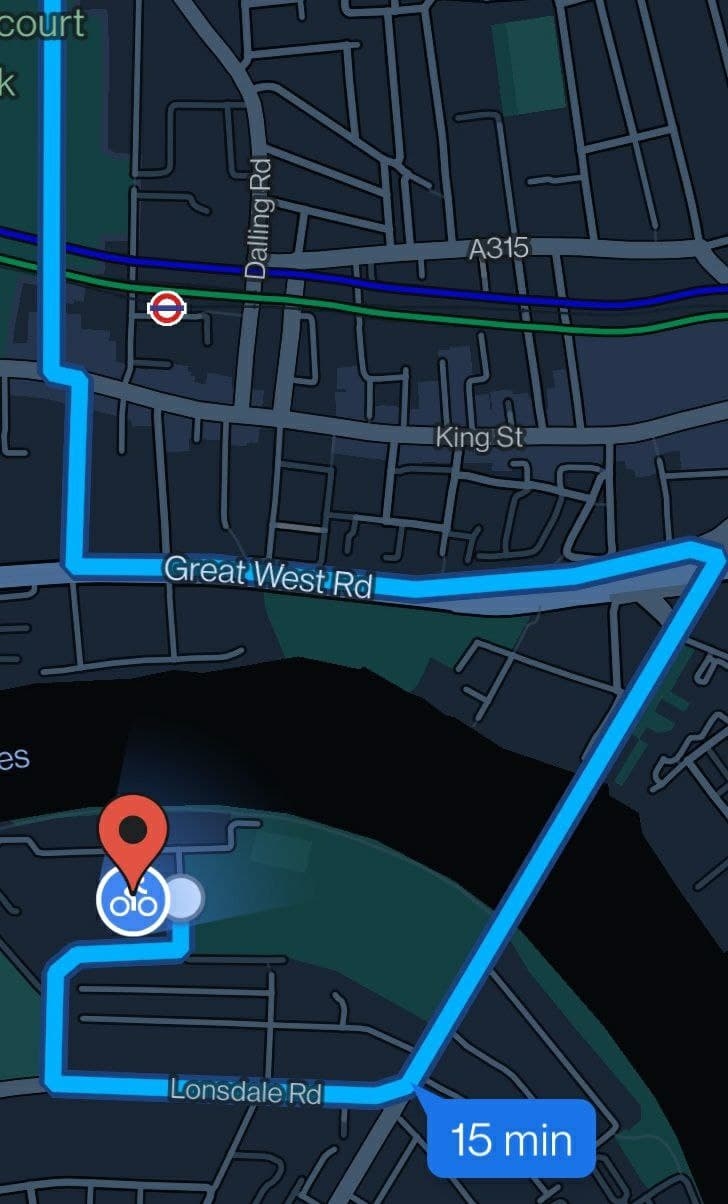
\includegraphics[height=5cm]{route.jpg}
    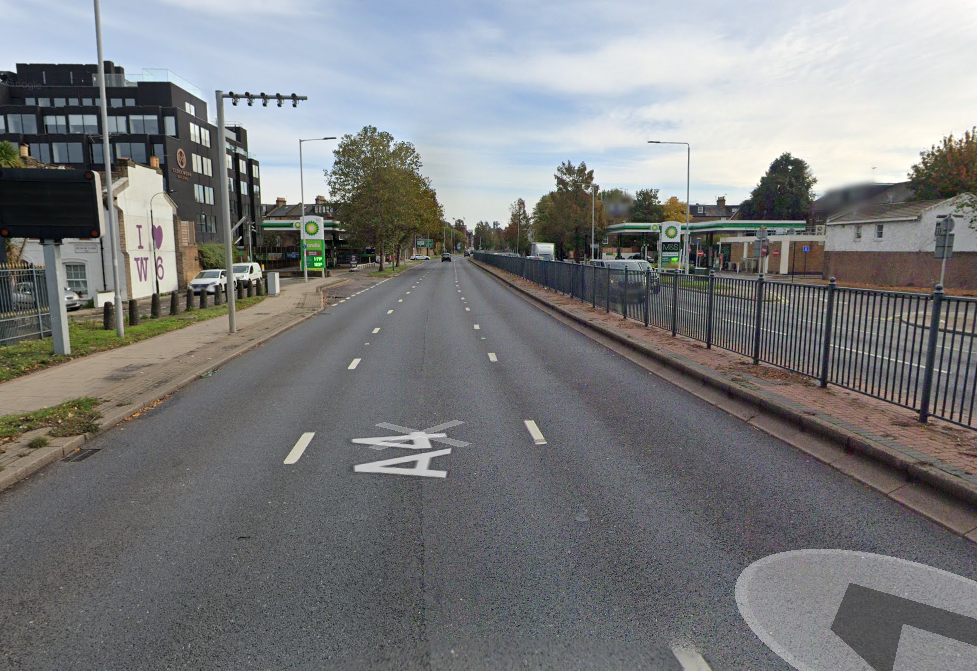
\includegraphics[height=5cm]{dangerous.png}
\end{center}
    \caption{Route suggested by google maps}
\label{route}
\end{figure}
Many of these route finding applications don't take into account safety considerations. This is shown in Figure \ref{route} which shows the route Google Maps suggests that I cycle to school by. The route includes the A4, which is a very dangerous stretch of road for cyclists as it is a 3 lane road. 
My plan is to use accident statistics to work out which roads are dangerous and then avoid them. This would be done by imposing a cost for going somewhere that there had been an accident.
\section{Client}
I interviewed Yuvraj Dubey, one of my classmates, to talk about whether they would be interested in a product that attempted to calculate safe routes to cycle. 
\begin{dialogue}
    \speak{Max}Do you own a bicycle?
    \speak{Yuvraj} Yes
    \speak{Max} Do you cycle regularly?
    \speak{Yuvraj} Yes
    \speak{Max}Do you ever feel in danger while cycling?
    \speak{Yuvraj}{Yes}
    \speak{Max}When do you feel in most danger while cycling?
    \speak{Yuvraj}At a Junction near Victoria, where there is a right turn and no cycle lane to do it in. I attempted to go this way once and was almost hit by a bus.
    \speak{Max}Are you aware of your surroundings while cycling?
    \speak{Yuvraj}Not really
    \speak{Max} Do you feel aware of the places which to cycle in safely, does this change when you are in places you commonly go?
    \speak{Yuvraj}No, but especially where I don't know where I am because then I do not know where it is safe to cycle. When I cycle home I have learnt a safe route, but if asked to cycle somewhere I did not know I would most likely end up in a dangerous place.
    \speak{Max}Would you use an application that tells you safe routes to get places?
    \speak{Yuvraj}Yes
    \speak{Max}Would you be happy using a command line application for this?
    \speak{Yuvraj}Yes
    \speak{Max}If said application took more than 60 seconds to calculate a route would you lose patience?
    \speak{Yuvraj}Yes, probably
    \speak{Max}Have you found that cycling directions generated by current products are safe and efficient?
    \speak{Yuvraj}They are definitely efficient, but they often take me onto busy roads and junctions which can be less safe.
\end{dialogue}
From this interview and my own experiences cycling in London I determined that there was an application for my idea, but only if it ran in a reasonable amount of time and was otherwise easy to use, as people struggle to find safe routes themselves, especially when going somewhere they had not previously been, and commercial
products such as Google Maps don't generate safe routes. 
\textcolor{red}{Add a little bit more analysis to this bit}
\newpage
\section{Similar Systems}
\begin{figure}[h]
    \begin{center}
        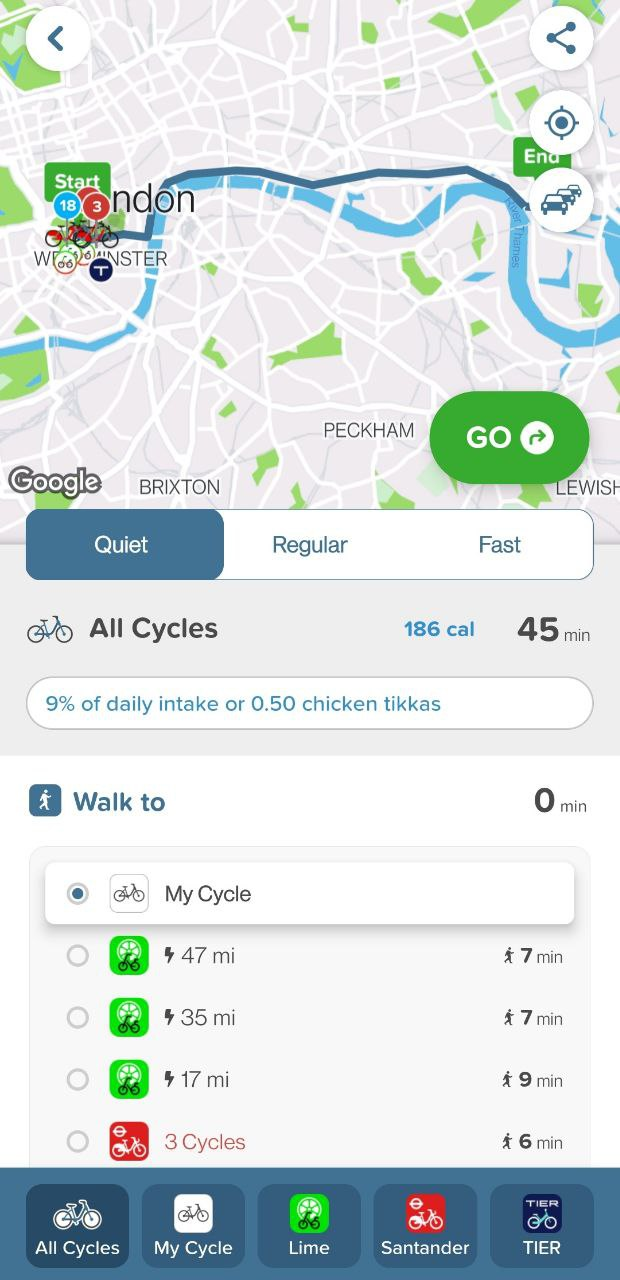
\includegraphics[height=10cm]{citymapper.png}
    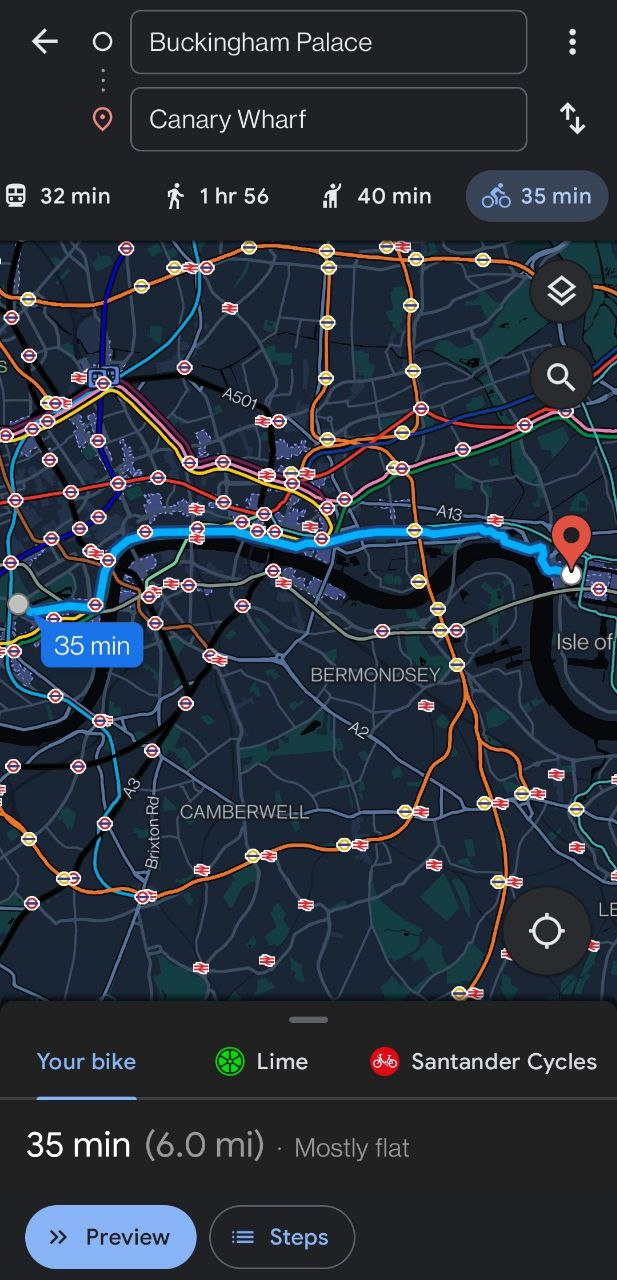
\includegraphics[height=10cm]{googlemaps.png}
\end{center}
    \caption{Citymapper and Google Maps respectively, generating the same directions}
    \label{alternatives}
\end{figure}
There exist similar systems for route finding such as Google Maps and Citymapper. These have advantage's over what I will be able to offer such as being able to use live traffic data, and having a good user interface. Citymapper has a option to choose between "Quiet", "Regular", and "Fast" routes, which seems to be based on the type of road you are taken down.
However they don't really take accident density into account which will be my aims.
\section{Features}
\subsection{Map data}
I need a data source which can provide data on roads that are legal to cycle on as well as being freely available for me to use. I settled on Open Street Map, a project which combines data gathered by volunteers into one massive freely available map. The map is downloadable in the form of a large XML file or PBF file. A PBF file is just a binary version of the same thing. I will write code to parse one of these myself.

\subsection{Accident Data}
\begin{figure}
    \begin{center}
        \begin{tikzpicture}[scale=1]
        \draw[gray, thick] (-4,0) -- (4,0);
        \draw[gray, thick] (0,-4) -- (0,4);
        \filldraw[black] (0,0) circle (2pt) node[anchor=west]{};
        \filldraw[black] (0,2) circle (2pt) node[anchor=west]{};
        \filldraw[black] (2,0) circle (2pt) node[anchor=west]{};
        \filldraw[black] (-2,0) circle (2pt) node[anchor=west]{};
        \filldraw[black] (0,-2) circle (2pt) node[anchor=west]{};
\filldraw[black] (0,-4) circle (2pt) node[anchor=west]{};
\filldraw[black] (0,4) circle (2pt) node[anchor=west]{};
\filldraw[black] (4,0) circle (2pt) node[anchor=west]{};
\filldraw[black] (-4,0) circle (2pt) node[anchor=west]{};
    \end{tikzpicture}
\end{center}
    \caption{Typical OSM representation of an intersection}
    \label{intersection}
\end{figure}
Transport for London has an excellent API which you can download accident data from. The data comes in JSON files and contains information about what type of vehicle was involved in each accident, the severity, and the coordinates of the accident. 
I need to find a way of mapping the coordinates onto the road network so that the danger of roads can be calculated as accurately as possible. Originally I was looking at adding the accident to the nearest edge in the graph but I decided against this after considering how intersections 
are typically represented in OSM. Road intersections typically look something like what is represented in Figure \ref{intersection}. If an accident were to occur at the intersection it would end up being added to one of the segments leading into the intersection, so the danger would not be properly calculated if not passing through that segment. Instead I thought about adding the danger to the nearest node, so that the accident would always be counted when a route passes through that intersection.
The other problem that I have to deal with, if adding data to the nearest node is that the density of nodes is not constant. Straighter roads will not need to use as many OSM nodes as curved roads, so i might incorrectly add cost to the wrong node. My proposed solution to this is to interpolate in nodes to a very high density to deal with this problem.
\subsection{Traffic Data}
The main problem with this is that the accident data is absolute and can thus not be used to calculate probabilities. For example, more accidents happen on King's Street than the dangerous road I showed earlier, but this doesn't mean that King's Street is more dangerous merely that more cyclists travel on it. This means that I need to get accurate cyclist traffic data for the whole of London in order to turn my accident statistics into accident probabilities.
The Department for Transport and the Office for National Statistics both keep data on traffic, but it isn't applicable because cycle data is only given as a total \footnote{0.6 billion miles per year in London} and at specific count points.
This means that I will either need to work out traffic data or get it from some dataset, such as Strava's Global Heatmap. \\
Luckily the rest of the application can work without including traffic data so my plan is to deal with this problem at a later time or hope that the avoidance of accidents alone will be enough.  
\subsection{Finding the shortest route}
Algorithms for finding the shortest path in a Graph are abundant. The most well known is Dijkstra's algorithm, and it's variant A*. In large Graphs, both Dijkstra's algorithm and A* can be very slow. I will most likely use preprocessing based algorithms such as ALT*/Contraction Hierachies to make my program run a lot faster.
This preprocessing will take a long time, but when completed it will significantly reduce the time taken to complete searches. 
\section{Class Layout}
\begin{figure}[t]
    \begin{center}
    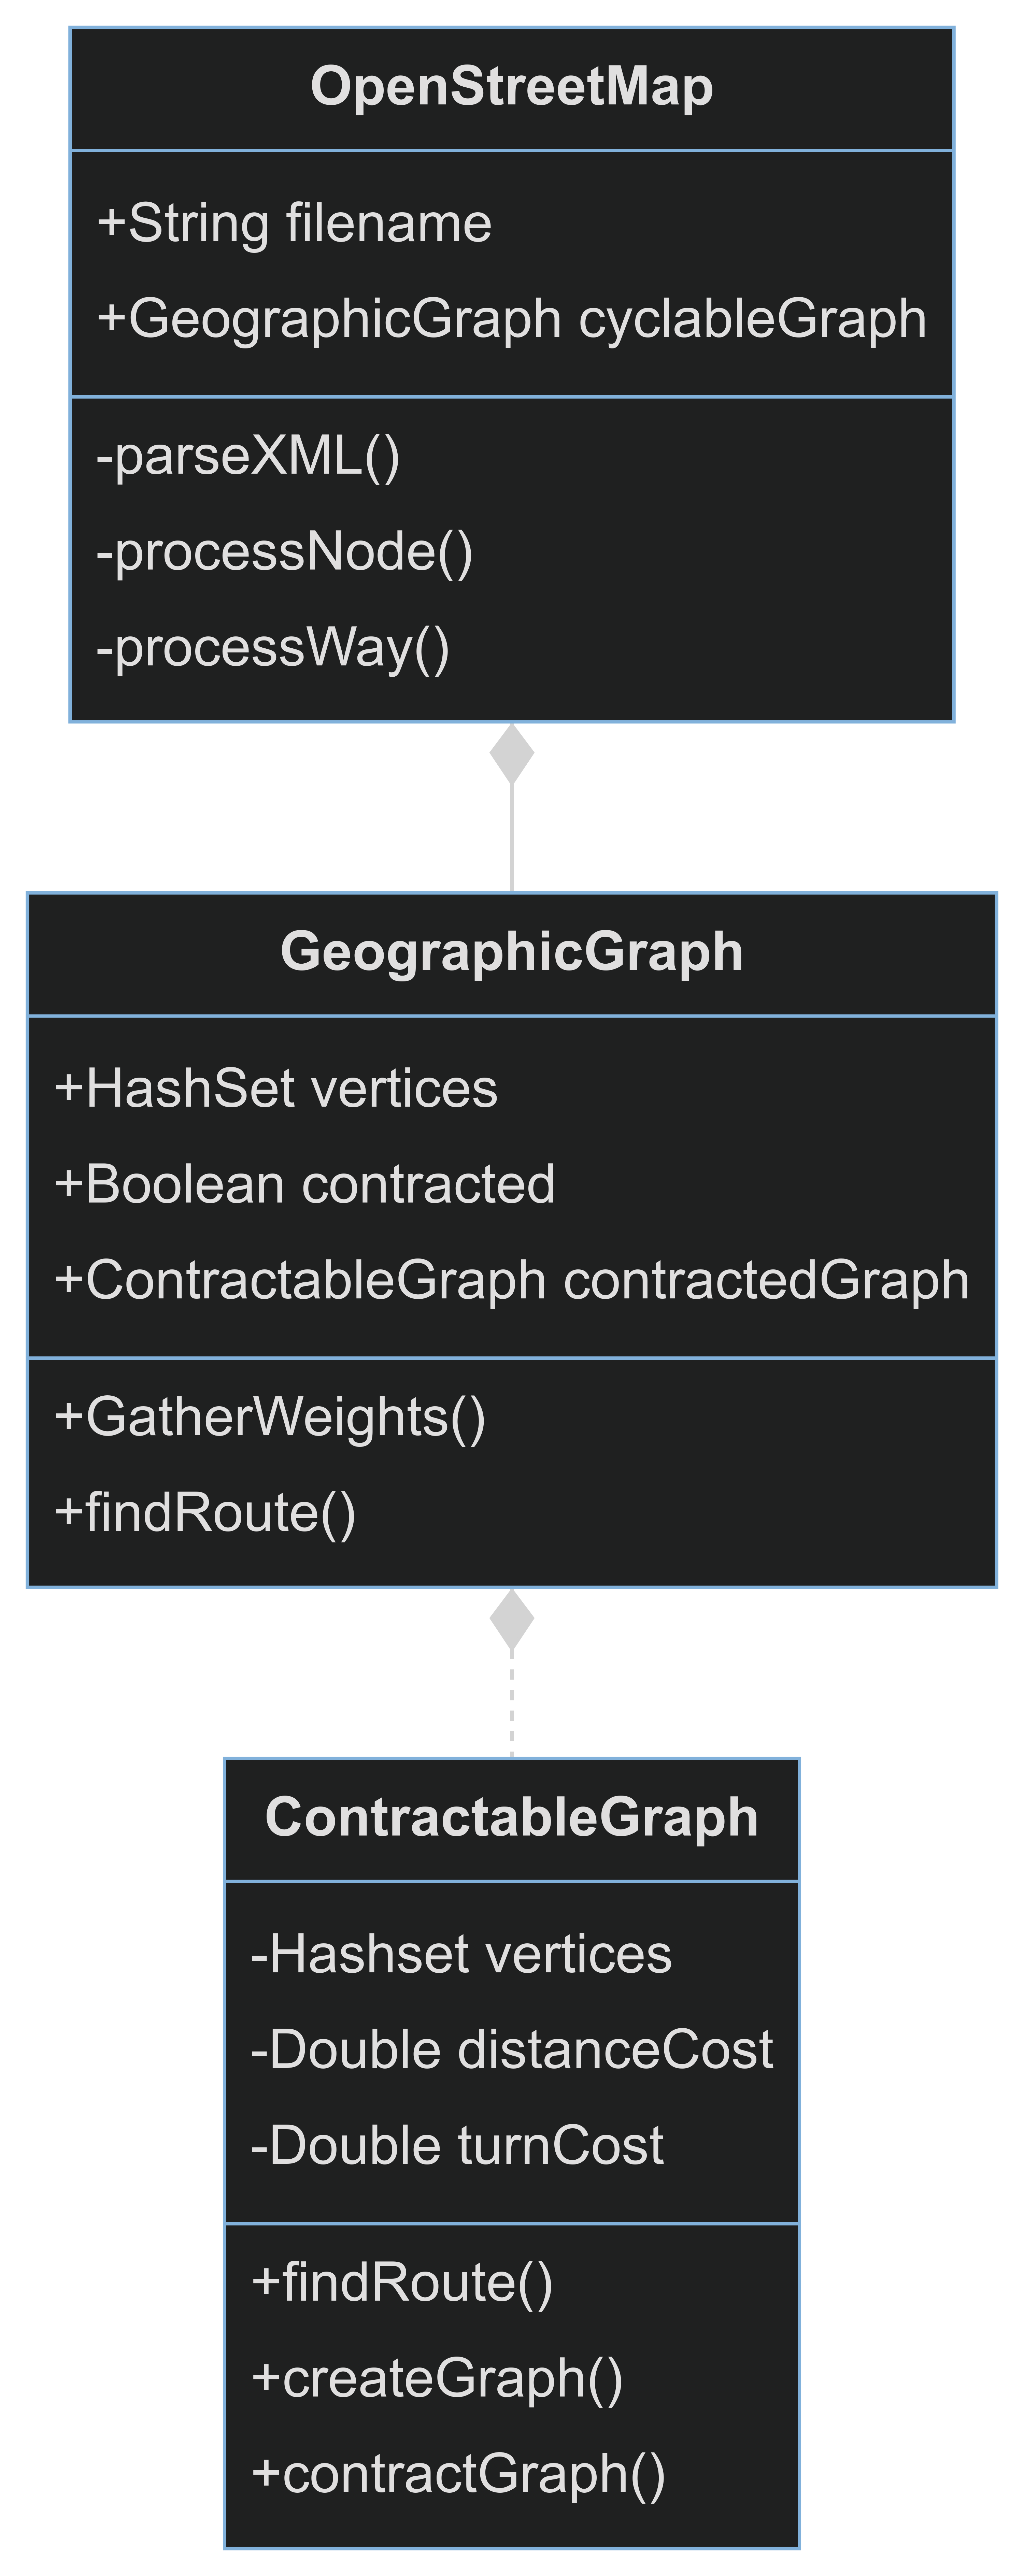
\includegraphics[height=8cm]{classdiagram.png}
    \end{center}
    \caption{Rough idea of the class diagram I will use}
    \label{Class Diagram Simple}
\end{figure}
As seen in Figure \ref{Class Diagram Simple}, I think I will use 3 major classes which will deal with parsing, storing, and preprocessing Graph data respectively. These will be linked by object composition
rather than inheritance. Where possible I will use private fields and methods. 
\section{Critical Path}
\begin{itemize} 
    \item Download accidents from the TFL API, parse for accidents that are of interest, and store it in a format that can be easily parsed later
    \item Import OSM map of London as a Graph which can be easily queried.
    \item Write code that imports the accident data and connects it to given Graph nodes.
    \item Write a simple Dijkstra's Algorithm method of finding the shortest path.
    \item Write a preprocessing based method of finding the shortest path.
    \item Write a frontend for the input of user options.
\end{itemize}
\newpage
\section{Specification}
\begin{enumerate}
\item Accident Download System
\begin{enumerate}[label=\arabic{enumi}.\arabic*]
    \item \label{downloadaccidents}The System must be capable of interfacing with the TFL API to download accidents
    \item \label{parseaccidents}The System must be capable of parsing accident data to determine which accidents are relevant
    \item \label{storeaccidents}The System must be capable of storing accident data in a easily accessible file for the route finding algorithm to parse
\end{enumerate} 
\item Route Finding System
\begin{enumerate}[label=\arabic{enumi}.\arabic*]
    \item \label{item-one} The System should be capable of processing an Open Street Map map file into a suitable data structure
    \item \label{item-two}The System should be capable of processing the accident data from the Accident Download System
    \item \label{item-three}The System should be capable of attaching the data from the Accident Download System to the suitable data structure from specification point \ref{item-one}
    \item \label{item-four}The System should be capable of using Accident Data combined with other suitable cost estimation functions to find a directed route between two points that are places on roads in London
    \item \label{item-five}The System should always suggest a route that can be followed while observing all currently known laws of physics
    \item \label{item-six}The System should always suggest a route that can be followed while observing all international, national, local laws and all releveant bylaws
    \item \label{item-seven}The System should suggest a safe route wherever possible
    \item \label{item-eight}The System should have guards in place for certain types of roads which are deemed too dangerous to consider
    \item \label{item-nine}The System should be able to generate this route quickly
    \item \label{item-ten}The System should have a mode for preprocessing to make the route generation even quicker
    \item \label{item-eleven}When using the same parameters, the route generated using a preprocessed graph and associated algorithms should be the same as that generated by the non-preprocessing based approach
    \item \label{item-twelve}The System should be easy to use
    \item \label{nocrashy} \label{item-thirteen}The System should not crash, and should give appropriate non crashing errors if user data is determined to be bad
    \item \label{item-fourteen} The parameters for the cost estimation functions should be user definable, but sensible defaults should also be defined
    \item \label{item-fifteen}\label{followpossible}The Route should be output in a format that is easy for the user to follow on a mobile device
    \item \label{item-sixteen}The System should have a system for saving all data from intensive calculation to disk
\end{enumerate}
\end{enumerate}
\newpage
\section{Specification Justification}
\begin{enumerate}
    \item Accident Download System
    \begin{enumerate}
        \item This point is required in order to obtain the necessary accident data
        \item This point is required to reduce the file sizes needed to be packaged with the project, and make it easier to use later
        \item This point is required as otherwise the system would not do much good in making the Route Finding System simpler
    \end{enumerate} 
    \item Route Finding System
    \begin{enumerate}
        \item The suitable data structure is required for all further queries
        \item The accident data is required for route finding applications
        \item This is required to tell where the costs for the accidents should be applied in shortest path queries
        \item This is the main function of the project; if it can't do that it will be worthless
        \item The Route should be realistic and connected; it can't ask people to teleport to their destination or phase through walls
        \item The Route should only take people onto roads which are publicly accessible and legal to cycle on, as obviously I do not want to encourage people to break laws
        \item The Route should attempt to be as safe as possible. Of course in some situations there is only one route which could be unsafe. In that situation that route would be suggested
        \item Some roads can be very dangerous to cyclists, such as canal paths, and these won't necessarily be represented through the data
        \item If the route generation takes too long the user will get bored. Other products offering the same features can generate routes very quickly
        \item London is very large, and route generation may be slow without preprocessing, so the preprocessing mode will help with that
        \item This makes sure that the preprocessing based approach is not losing information about the best route in any way
        \item If the system was not easy to use, people would not use it
        \item This feeds into the previous specification point
        \item The customisability would allow users to make their own decisions about tradeoffs between time and safety, and sensible defaults should generate sensible routes
        \item Especially with longer routes, the probability of the user being able to remember the route is slim, so they will need a mobile device to be able to guide them
        \item The parsing of XML files may take a while, and the preprocessing for query speedup definitely will. If the results of this can be saved to disk repeating this every time the program is run will not be necessary.
    \end{enumerate}
\end{enumerate}
\newpage
\chapter{Design}
\section{Accident Download System}
As outlined in the Specification, this system should be capable of interfacing with the TFL API, downloading the accidents, deciding which ones are relevant, and storing this in a useful format.
\subsection{Pulling from the TFL API}
\label{Pulling from the TFL API}
The Transport For London API is an excellent API which can provide information on many different aspects of the Transport For London network. The specific API which I used is the AccidentStats API.
This API is very simple, you simply request a given year and a JSON object is returned which contains all of the accidents that happened in london that year. These consist of all the accidents that were reported tocdepth
the police as happening in that year. Of course, there will be many more accidents than are on the API, but these will mostly be more minor accidents.
The Data is returned as a list of accidents, formatted as shown in Figure \ref{Default}.
\begin{figure}[t]
\begin{lstlisting}[language=Python]
[{
    "id": 0,
    "lat": 0.0,
    "lon": 0.0,
    "location": "string",
    "date": "string",
    "severity": "string",
    "borough": "string",
    "casualties": [{
        "age": 0,
        "class": "string",
        "severity": "string",
        "mode": "string",
        "ageBand": "string"
    }],
    "vehicles": [{
        "type": "string"
    }]
}]
    \end{lstlisting}
\caption{The Default output from the API \cite{tflapi}}
\label{Default}
\end{figure}
\\
As the data about accidents that happened in the past is not going to change any time soon, and TFL only updates this API every year, it is simplest just to download the files once, parse it once, and then 
use that result in the route finder. I used two scripts to do this.\\
TFL started gathering this data in 2005, and the most recent update was in 2019, so the first script downloads all the data from 2005 to 2019 and save it in a subfolder called \texttt{accidents}.
The script loops through all the years between 2005 and 2019 and creates a JSON file for that year. \\
\subsection{Parsing the Data}
The next step is to go through the data from all the years\footnote{I later decided to remove some years see Section \ref{Accident Download System Implementation}}, and save all the accidents that are pertinent to my project. As seen in Figure \ref{Default}, each accident listing has information on casualties,\\
of which there may be many. As this is a cycling application, I only want data on accidents where at least one of the casualties was a cyclist. The API provides a lot of data, but all that is relevant is
the latitude and longitude, as well as the severity of the incident. All of this data was ultimately saved to a file called \texttt{output.json}.
 The intended format of the file data will be saved in is shown in Figure \ref{accident format}.
\begin{figure}[t]
\begin{lstlisting}[language=Python]
[
    ["Latitude","Longitude","Severity"]
]
\end{lstlisting}
\caption{Intended format for parsed accident file}
\label{accident format}
\end{figure}
\newpage
\section{Route Finding System}
\subsection{Overview and Design Choices}

\begin{figure}[p]
    \begin{center}
        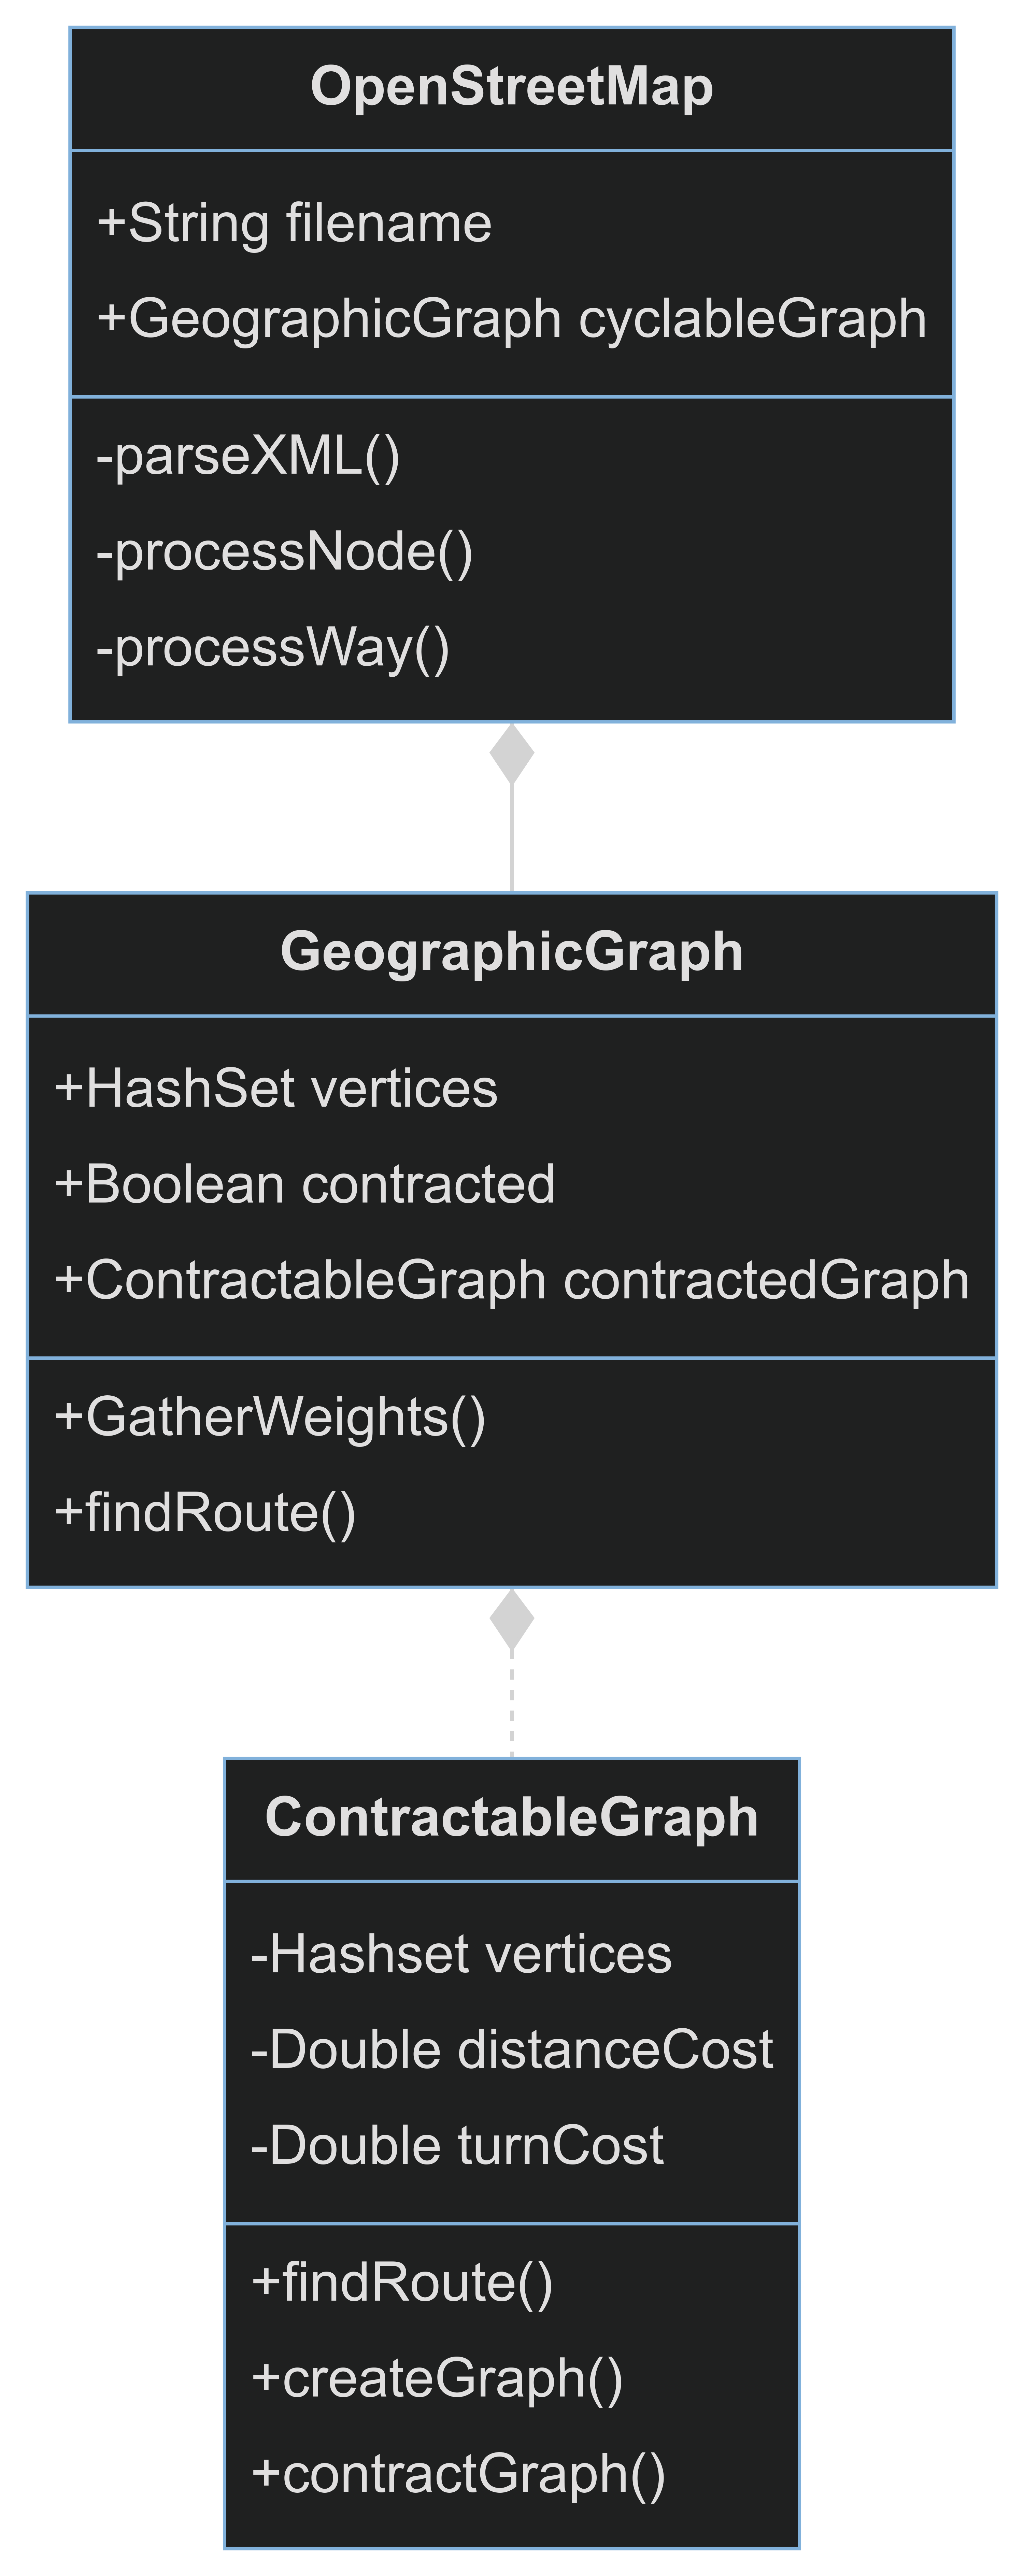
\includegraphics[height=21cm]{classdiagram.png}
    \end{center}
    \caption{Rough UML diagram for the project}
    \label{uml}
\end{figure}
I decided to use Kotlin for this project. Kotlin is related to Java in that it allows access to all the Standard Java Libraries, as well
as external ones, and it runs in the Java Virtual Machine. Kotlin does not need to maintain backwards compatability with old Java code,
so it has a much cleaner API and has nice syntax. As this was a new project not dependent on using Java code Kotlin was an obvious choice. 
Furthermore, Java code can be easily translated into Kotlin code, so I could code things in Java then translate over if necessary. Like Java, kotlin allows Object-Oriented-Programming, so that
is the approach I will be taking in this project.\\
As seen in Figure \ref{uml}, I decided to define 3 main classes for my NEA. \texttt{OpenStreetMap} contains methods for parsing OSM files and creating a graph.
\texttt{OpenStreetMap} contains a single instance of the \texttt{GeographicGraph} class by object composition. This is because there will only be one \texttt{GeographicGraph}
class associated with a given OSM file, and this system could be easily extended to hold information on two separate graph areas at the same time, which could be used if I wanted
to extend the system to more cities. The \texttt{GeographicGraph} can contain an instance of the \texttt{ContractableGraph} class, if it has been contracted. If it has not been contracted,
this class will not exist.\\
I also created two other classes, \texttt{IntTuple} and \texttt{DoubleTuple}, which are used in priority queues in both the \texttt{GeographicGraph} and \texttt{ContractableGraph} classes.\\
\subsection{Open Street Map Data}
Open Street Map is a world map generated by user mapping. It contains multitudes of data on all sorts of mappable things, from the height of stories to the roads that encompass them.
Files can be in one of two formats; PBF \footnote{Protocol Buffer Format} which is a highly efficient binary format, and XML\footnote{Extensible Markup Language} which is a markdown language. I tried to use a library to parse 
the PBF file into a Graph, but the main library for that did not work. So instead I decided to parse it manually as an XML file.\\
\subsubsection{Getting the relevant file}
Openstreetmap has an API for requesting parts of the map, but it does not allow requesting large areas, such as the whole of London. There are many mirrors from which you can download large parts of the world. I decided to use geofabrik \cite{geofabrik}
 because it allows you to download single countries. Next I extracted London from this dataset. This is not strictly necessary, as my program can still deal with large areas such as the whole of the UK, but it does not have accident data for such an area.
 Furthermore it would increase the file size needed on disk and increase the running time of any preprocessing. In order to extract London, I used a GeoJSON\cite{geojsondefinition} file, which is essentially a list of coordinates. I found a GeoJSON file on the internet \cite{geojsonsource}
 of the M25 boundary, and used the following command\footnote{I used the OSM manipulation tool Osmium} to cut out London: 
 \begin{verbatim}
$osmium extract -p course_m25_boundary.json united_kingdom.osm.pbf -o london.osm
 \end{verbatim}
 This file could be used by my program, as it intelligently avoids parsing non-routable ways and, but I decided to further reduce the file size by removing all nodes and ways that were not part of highways.
 This was just for quality of life, as it makes parsing the file much faster.
 \begin{verbatim}
$osmium tags-filter london.osm nw/highway -o ways.osm
 \end{verbatim}
 This created a 370MB file called \texttt{ways.osm}. I could have reduced this further by removing the ways that are irrelevant to the program, but I decided to do that in the parser so that it would be
 more easily configurable.
\subsubsection{Parsing the file}
Open Street Map files are built out of 3 main elements \cite{osmwikipage}:
\begin{itemize}
    \item Nodes, which contain longitude and latitude. 
    \item Ways, which contain between 2 and 2000 ordered nodes. These are used to form roads, but also all kinds of other polygons, such as buildings, rivers, and walls. 
    \item Relations, which contain many ways, nodes and relations. These are used to connect things together, like all roads on a certain bus route. These are not relevant to my project.
\end{itemize}
All of these elements can also contain additional information on what type of node or way it is, as well as a unique id. 
As I only care about nodes that are part of roads I can ignore the relation element completely. In a \texttt{.osm} file, the nodes all come first. This means that I can parse the nodes, 
and then figure out how all the nodes are connected using the ways.\\
\begin{figure}[t]
    \begin{lstlisting}[language=XML]
<way id="1202" version="32" timestamp="2019-05-15T08:24:07Z" uid="7105697" user="_Garrison_" changeset="70264933">
    <nd ref="5335693253"/>
    <nd ref="5335693250"/>
    <nd ref="104429"/>
    <nd ref="3330244696"/>
    <nd ref="5335691516"/>
    <tag k="bicycle" v="no"/>
    <tag k="foot" v="no"/>
    <tag k="highway" v="trunk"/>
    <tag k="horse" v="no"/>
    <tag k="lanes" v="3"/>
    <tag k="lit" v="yes"/>
    <tag k="maxspeed" v="40 mph"/>
    <tag k="maxspeed:enforcement" v="average"/>
    <tag k="name" v="North Circular Road"/>
    <tag k="oneway" v="yes"/>
    <tag k="operator" v="Transport for London"/>
    <tag k="ref" v="A406"/>
    <tag k="sidewalk" v="none"/>
    <tag k="surface" v="asphalt"/>
</way>
\end{lstlisting}
\caption{One of the Ways in \texttt{ways.osm} extracted}
\label{North Circular}
\end{figure}
After some research, I determined that the best way to parse the XML was to use the library \texttt{dom4j} \cite{dom4jsite}. I decided that the \texttt{OpenStreetMap} class needs 3 functions: \texttt{parseXML}, \texttt{processNode}, and \texttt{processWay}.
The function that is called with the direct input file is \texttt{.parseXML} 
Essentially what it does is iterate through the items in the XML file, calling either \texttt{processNode} or \texttt{processWay}. \texttt{processNode} simply adds a new node to the \texttt{GeographicGraph}.
The \texttt{processWay} function is more complex as it has to work out whether ways should be added to the graph, and if additional data needs to be stored about them. Within each way stored in the \texttt{.osm} file,
there will be additional tags that hold more data about the way \cite{osmhighwayspage}. An example way, which is part of the North Circular road, is shown in Figure \ref{North Circular}.\\
First there are a ordered list of nodes which are sequentially connected, then there is a collection of optional Key Value pairs which form tags. The \texttt{processWay}
function analyzes these tags in order to determine if the road is acceptable for cyclists. The example in Figure  \ref{North Circular}
would probably not be a good way to include, because the tag \texttt{bicycle} is set to \texttt{no}, and it is a 3 lane road with a 40mph speed limit. The progam uses 
accident data to work out which roads are dangerous, but some roads will not have many accidents on them simply because they are so dangerous nobody would ever cycle on them. 
\paragraph{Parsing the ways}
In order to convert from XML to a data representation in memory, we simply iterate through all the subelements in the way. If it is a reference to a node, the id is appended to a ordered list,
and if it is a tag, it is added to a HashMap so it can be more easily queried. 
\paragraph{Deciding what is allowed}
\begin{itemize}
    \item Highway tag
    \begin{itemize}
        \item This tag is present in all roads mapped in OSM, so it's presence must be checked for.
        \item This tag represents the \say{the importance of the highway within the road network as a whole}\cite{osmhighwayspage}.
        \item This does not normally represent anything about the road quality, safety, usage, layout, or maximum speed. The exceptions to this are
        \begin{itemize}
            \item \texttt{motorway} which is obviously not wanted.
            \item \texttt{living\_street} which represents places where pedestrians and cyclists have legal priority, such as Low Traffic Neighbourhoods.
            \item \texttt{cycleway} which encompasses segregated areas for cyclists. 
            \item \texttt{bridleway} which is a segregated area for horses, where cyclists may be allowed.
            \item \texttt{footway} which is a footpath which cannot be cycled on.
        \end{itemize}
    \end{itemize}
    \item Access tag. This tag represents what the access arangements for the area in question are. If it is \texttt{no} or \texttt{private}, the way would not be wanted.
    \item Bicycle and Motor tags. These tags are the same as the access tag, but for specific types of vehicle.
    \item Surface tag. This represents the surface the route is made out of. Ways that are made out of dirt or similar materials will not be parsed.
    \item Note tag. This can contain lots of different notes, but the one \texttt{processWay} looks for is the \texttt{towpath}, as these can be dangerous in a way that is not represented in the TFL accident data
    \item Oneway tag. If true, the route will only be connected oneway.
    \item Maxpseed tag. This can be used to exclude dangerous roads.
\end{itemize}
After analyzing these tags \texttt{processWay} has multiple outcomes.
\begin{itemize}
    \item Way is included in the graph in both directions.
    \item Way is included in the graph only in the same direction as the ordered list of nodes, because \texttt{oneway} is set to \texttt{yes}.
    \item Way is considered too dangerous to include or access to cyclists is not guaranteed to be legal so specification point \ref{item-five} would not be followed.
    \item Way is included in the graph and the nodes are added to a set of safe nodes because it is in a cycle route or footpath.
    \item Way is included in the graph and the nodes are added to a set of nodes that will be slower to travel on because of a footpath.
\end{itemize}
Some of these outcomes can overlap, such as being added to the group of safe nodes and having edges only added in one direction.\\
\begin{enumerate}
    \item The way is parsed in some form if:
    \subitem The \texttt{highway} value is not null, and is within a set of allowed highway types
    \subitem The \texttt{access} and \texttt{bicycle}\footnote{In places where cycling is not permitted but walking with a bike is this will be dismount instead of no} value are not within a set of disallowed access types.
    \subitem The \texttt{surface} value is not within a list of disallowed surfaces
    \subitem The \texttt{maxspeed} value is not more than 30 miles per hour
    \subitem The \texttt{note} value does not say that the path is a towpath
    \item The way is only parsed in one direction if:
    \subitem The \texttt{oneway} tag is set to yes
    \item The way is marked as a safe node if it is
    \subitem Marked as a \texttt{cycleway}, \texttt{footway} ,or \texttt{pedestrian} or \texttt{motor\_vehicle} is set to private
    \item The way is marked as a slow way if it is 
    \subitem Marked as a \texttt{footway} or \texttt{pedestrian} and \texttt{bicycle} is not set to \texttt{designated}
\end{enumerate}
Of course, it will be very easy to iteratively develop this when the whole system is finished. If a certain way that looks like it should be routed down is not routed down or vice versa the function can be adjusted.
It is important to note that this function is designed to be quite open in deciding which ways are safe. It only excludes ways that are plainly very dangerous. The actual decision of where to go based on danger will be made by the
route finding algorithms.
\newpage
\subsection{Representing and Querying the Graph}
As shown in Figure \ref{uml}, my design uses a class called \texttt{GeographicGraph} to represent London\footnote{Other areas could be represented as well}. There are many graph libraries available to java programs, but creating my own implementation
 will allow me more flexibility in implementation of methods that relate to real world applications. As shown in Figure \ref{uml}, the \texttt{GeographicGraph} class has some major methods that need to be implemented. \texttt{gatherWeights} will 
 read in a accident file in the format specified in Figure \ref{accident format}, and attach the accident to the nearest node in the graph. \texttt{findRoute} will find the best route between two nodes in the graph.
There will also need to be other functions for maintaining and querying the data structure.
\subsubsection{Representing the Graph}
\label{Rtree}
There are many possible methods of representing Graphs, such as using an adjacency matrix, or an adjacency list. An adjacency matrix would not work in this case, as the graph is very sparse. An adjacency list could work, but maintaining information about the nodes 
separately from the adjacency list would be difficult. Instead, my design uses an OOP approach, where every relevant node in the OSM representation is converted into an equivalent node represented by a subclass called \texttt{GeographicNode}.
This is advantageous because it allows associated data, such as the number of accidents attached and the coordinates, to be stored in the same place. As shown in Figure \ref{geographicnode}, the connections would be represented as a HashSet. Ideally, this would contain
other \texttt{GeographicNode} objects that the node in question was connected to. However this would lead to problems with serialisation as explained in Section \ref{sec:serialization} so instead the unique ids from the OSM representation are used,
along with a lookup table for converting these back to \texttt{GeographicNode} objects.\\
Another feature that the \texttt{GeographicGraph} class needs to provide is facility for the conversion of coordinates to the id of the closest node. This will be useful for allowing the user to ask for directions in terms of coordinates,
as well as for attaching accidents to the nearest node.
In order to do this quickly and efficiently my design calls for the use of an R*Tree\cite{Beckmann1990}. This is a special type of data structure for holding coordinates that groups coordinates into a tree of rectangles. This allows much faster queries when looking for nodes that satisfy certain geometric properties, such as asking for the closest node.
The * in R*Tree means that a heuristic is used to try an optimise query times, by minimising overlap between rectangles. 
The implementation of an R*Tree is beyond the bounds of this project, and any I could implement would be less powerful than one from a library. To that end, I decided to use the library \texttt{rtree2}\cite{rtree}. I have used it in other projects before and found it to be very powerful. The R*-Tree will be set up when the graph is created, and a 
function called \texttt{getNearestNode} will convert between coordinates and OSM node ids. 
\begin{figure}[t]
    \begin{center}
        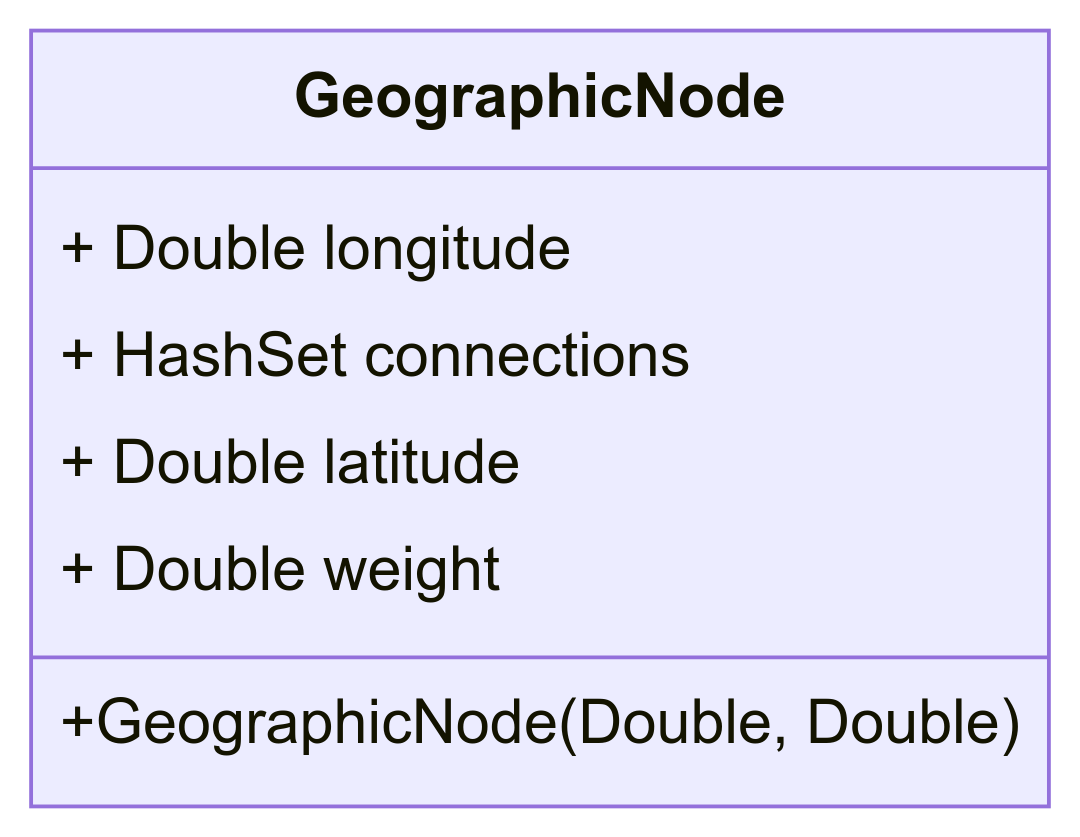
\includegraphics[width=8cm]{GeographicNode.png}
    \end{center}
    \caption{Rough UML class diagram for the \texttt{GeographicNode} subclass}
    \label{geographicnode}
\end{figure}
\subsubsection{Creating the Graph}
The \texttt{OpenStreetMap} class deals with parsing the XML, but it has to interface with the \texttt{GeographicGraph} class. When adding new nodes to the Graph, it can simply create a new instance of 
\texttt{GeographicNode} and add it to the relevant lookup table. For adding an edge, the functionality can be provided by a \texttt{addEdge} function. 
\paragraph{Pruning the Graph}
Due to the sequential order of parsing the OSM representation of the Graph, some nodes may be left disconnected because the way that connects them together was not parsed. If the system is asked to find a route from a 
node that is not connected to any other node, it will of course fail. This could lead to a crash, which would be in contravention of specification point \ref{nocrashy}, or at least a bad user experience, if given an error for seemingly sensible inputs.
Another problem could be that the Graph might have multiple components, perhaps because access to an area was cut off by safety protocols. Whatever the cause, both of these problems can be averted by removing all nodes that cannot be routed to by one location in the 
main component. This can be done by picking any node from which all other nodes can be connected to, finding the whole component, then removing any \texttt{GeographicNode} objects that are not in that component from the lookup table they are stored in. However there are two problems with this approach:
 the node that all other nodes are connected to must be picked manually, and the component is not guaranteed to be strongly connected. What this means is that while it is possible to reach any node in the component from the start node it is not necessarily for every node in the component. 
A component for which this would work is called a strongly connected component. If the function finds all strongly connected components and then assumes that the largest one is the one that is wanted the chance of allowing unsolvable queries is eliminated. 
One algorithm for finding all strongly connected components is Kosaraju's Algorithm\cite{wikipedia_2022}. This algorithm uses the fact that strongly connected components remain when all edges are reversed, and relies on a post-order DFS. The DFS is run first in the right direction, then in reverse to find the strongly connected components.
The following steps are followed.
\begin{lstlisting}
L <- []
visited <- []
FOR u in G:
    Visit(u)
Subroutine Visit(u):
    if u NOT IN visited:
        ADD u TO visited
        for each neighbour v:
            Visit(v)
        prepend u to L
FOR u in L:
    Assign(u,u)
Subroutine Assign(u,v):
    if u NOT assigned:
        assign u to v
        for each incoming neighbour p:
            Assign(p,v)
\end{lstlisting}
The ordering of L is important as it represents the direction in which connections are made in the components. These components are then checked to find the strongly connected components. Each strongly connected component will take a continuous region of L. 
Implementation of this may require modifying the \texttt{GeographicNode} class to also keep track of incoming connections.  
\subsubsection{Querying the Graph}
\begin{figure}[t]
    \begin{center}
\begin{lstlisting}
function Dijkstra(Graph, source, target):
     for each vertex v in Graph.Vertices:            
         dist[v] <- INFINITY                 
         prev[v] <- UNDEFINED                
         add v to Q                     
     dist[source] <- 0                           
     while Q is not empty:
          u <- vertex in Q with min dist[u]   
          remove u from Q
          if u == target: break                                        
          for each neighbor v of u still in Q:
              alt <- dist[u] + Graph.Edges(u, v)
              if alt < dist[v]:              
                  dist[v] <- alt
                  prev[v] <- u
  S <- empty sequence
  u <- target
  if prev[u] is defined or u = source:
      while u is defined:
         insert u at the beginning of S
         u <- prev[u]
\end{lstlisting}
\end{center}
\caption{Dijkstra's algorithm modified from Wikipedia\cite{dijkstrapseudo}}
\label{dijkstrapseudo}
\end{figure}
The main query that has to be provided for is finding the shortest route between two points. This functionality can be provided either by a simple Dijkstra's Algorithm implementation, or through a different query for the preprocessed Graph. If the graph has been preprocessed,
that mode should be used. Otherwise Dijkstra's shortest path algorithm should be used. 
\paragraph{Dijkstra's Algorithm}
Dijkstra's Algorithm\cite{Dijkstra1959} is a immensely popular algorithm for finding routes in graphs. It builds up a tree of nodes that it knows the shortest route to until said tree contains the target node. It does this by iterative "settling" of nodes.
The known unsettled node that has the shortest route cost to the start node is settled, and all of it's neighbours are added to a list of nodes to be settled. Every node has a tentative \texttt{dist} value and a tentative \texttt{prev} value, defined by the currently known shortest path to that route.
When the node is settled this value is known to be true. This process is repeated until the algorithm is completed. Pseudocode for Dijkstra's algorithm is shown in Figure \ref{dijkstrapseudo}. A Priority Queue can be used to find the next node to process. This is detailed in the Final Design section.
\\A variant of Dijkstra's algorithm called A*\cite{Hart1968} uses heuristics to reduce the required search space. The heuristic estimates the distance to the end node, meaning that nodes are vaguely settled in the right direction.
However this heuristic has to be "admissible" if the shortest possible route is to be found. This means that it never makes overestimates. As the density of accidents cannot be predicted between any point and the end node, the heuristic would be extremely loosely fitting, and would 
fail to significantly reduce the search space. 
\paragraph{Cost Function}
Any route finding algorithm needs a function or set of functions for the cost that would be incurred if going a certain way. If going from node $u$ to node $v$, the function $c$ would be:
\begin{align*}
    c(u,v) &= w(v) + a\times s(u,v)\times d(u,v) + b\times t(p(u),u,v)\\
    w(x) &= \operatorname{slight}(x) + 2 \times\operatorname{serious}(x) + 3\times\operatorname{fatal}(x)\\
    t(a,b,c) &=\begin{cases} \mbox{1} & \mbox{if } \angle abc < c \\ \mbox{0} & \mbox{otherwise} \end{cases}\\
    s(u,v) &=\begin{cases} \mbox{d} & \mbox{if } \text{both nodes are safe nodes} \\ \mbox{e} & \mbox{if both nodes are slow nodes}\\ \mbox{f} & \mbox{otherwise} \end{cases}\\
\end{align*}
where $a$,$b$,$c$,$d$,$e$,and $f$ are variables that can be tweaked. The turn function $t(a,b,c)$ can be used to impose a cost on turning too often, as this is makes routes harder to follow and increases danger. $\angle abc$ can be calculated 
using the cosine rule.
\begin{figure}[t]
    \begin{center}
    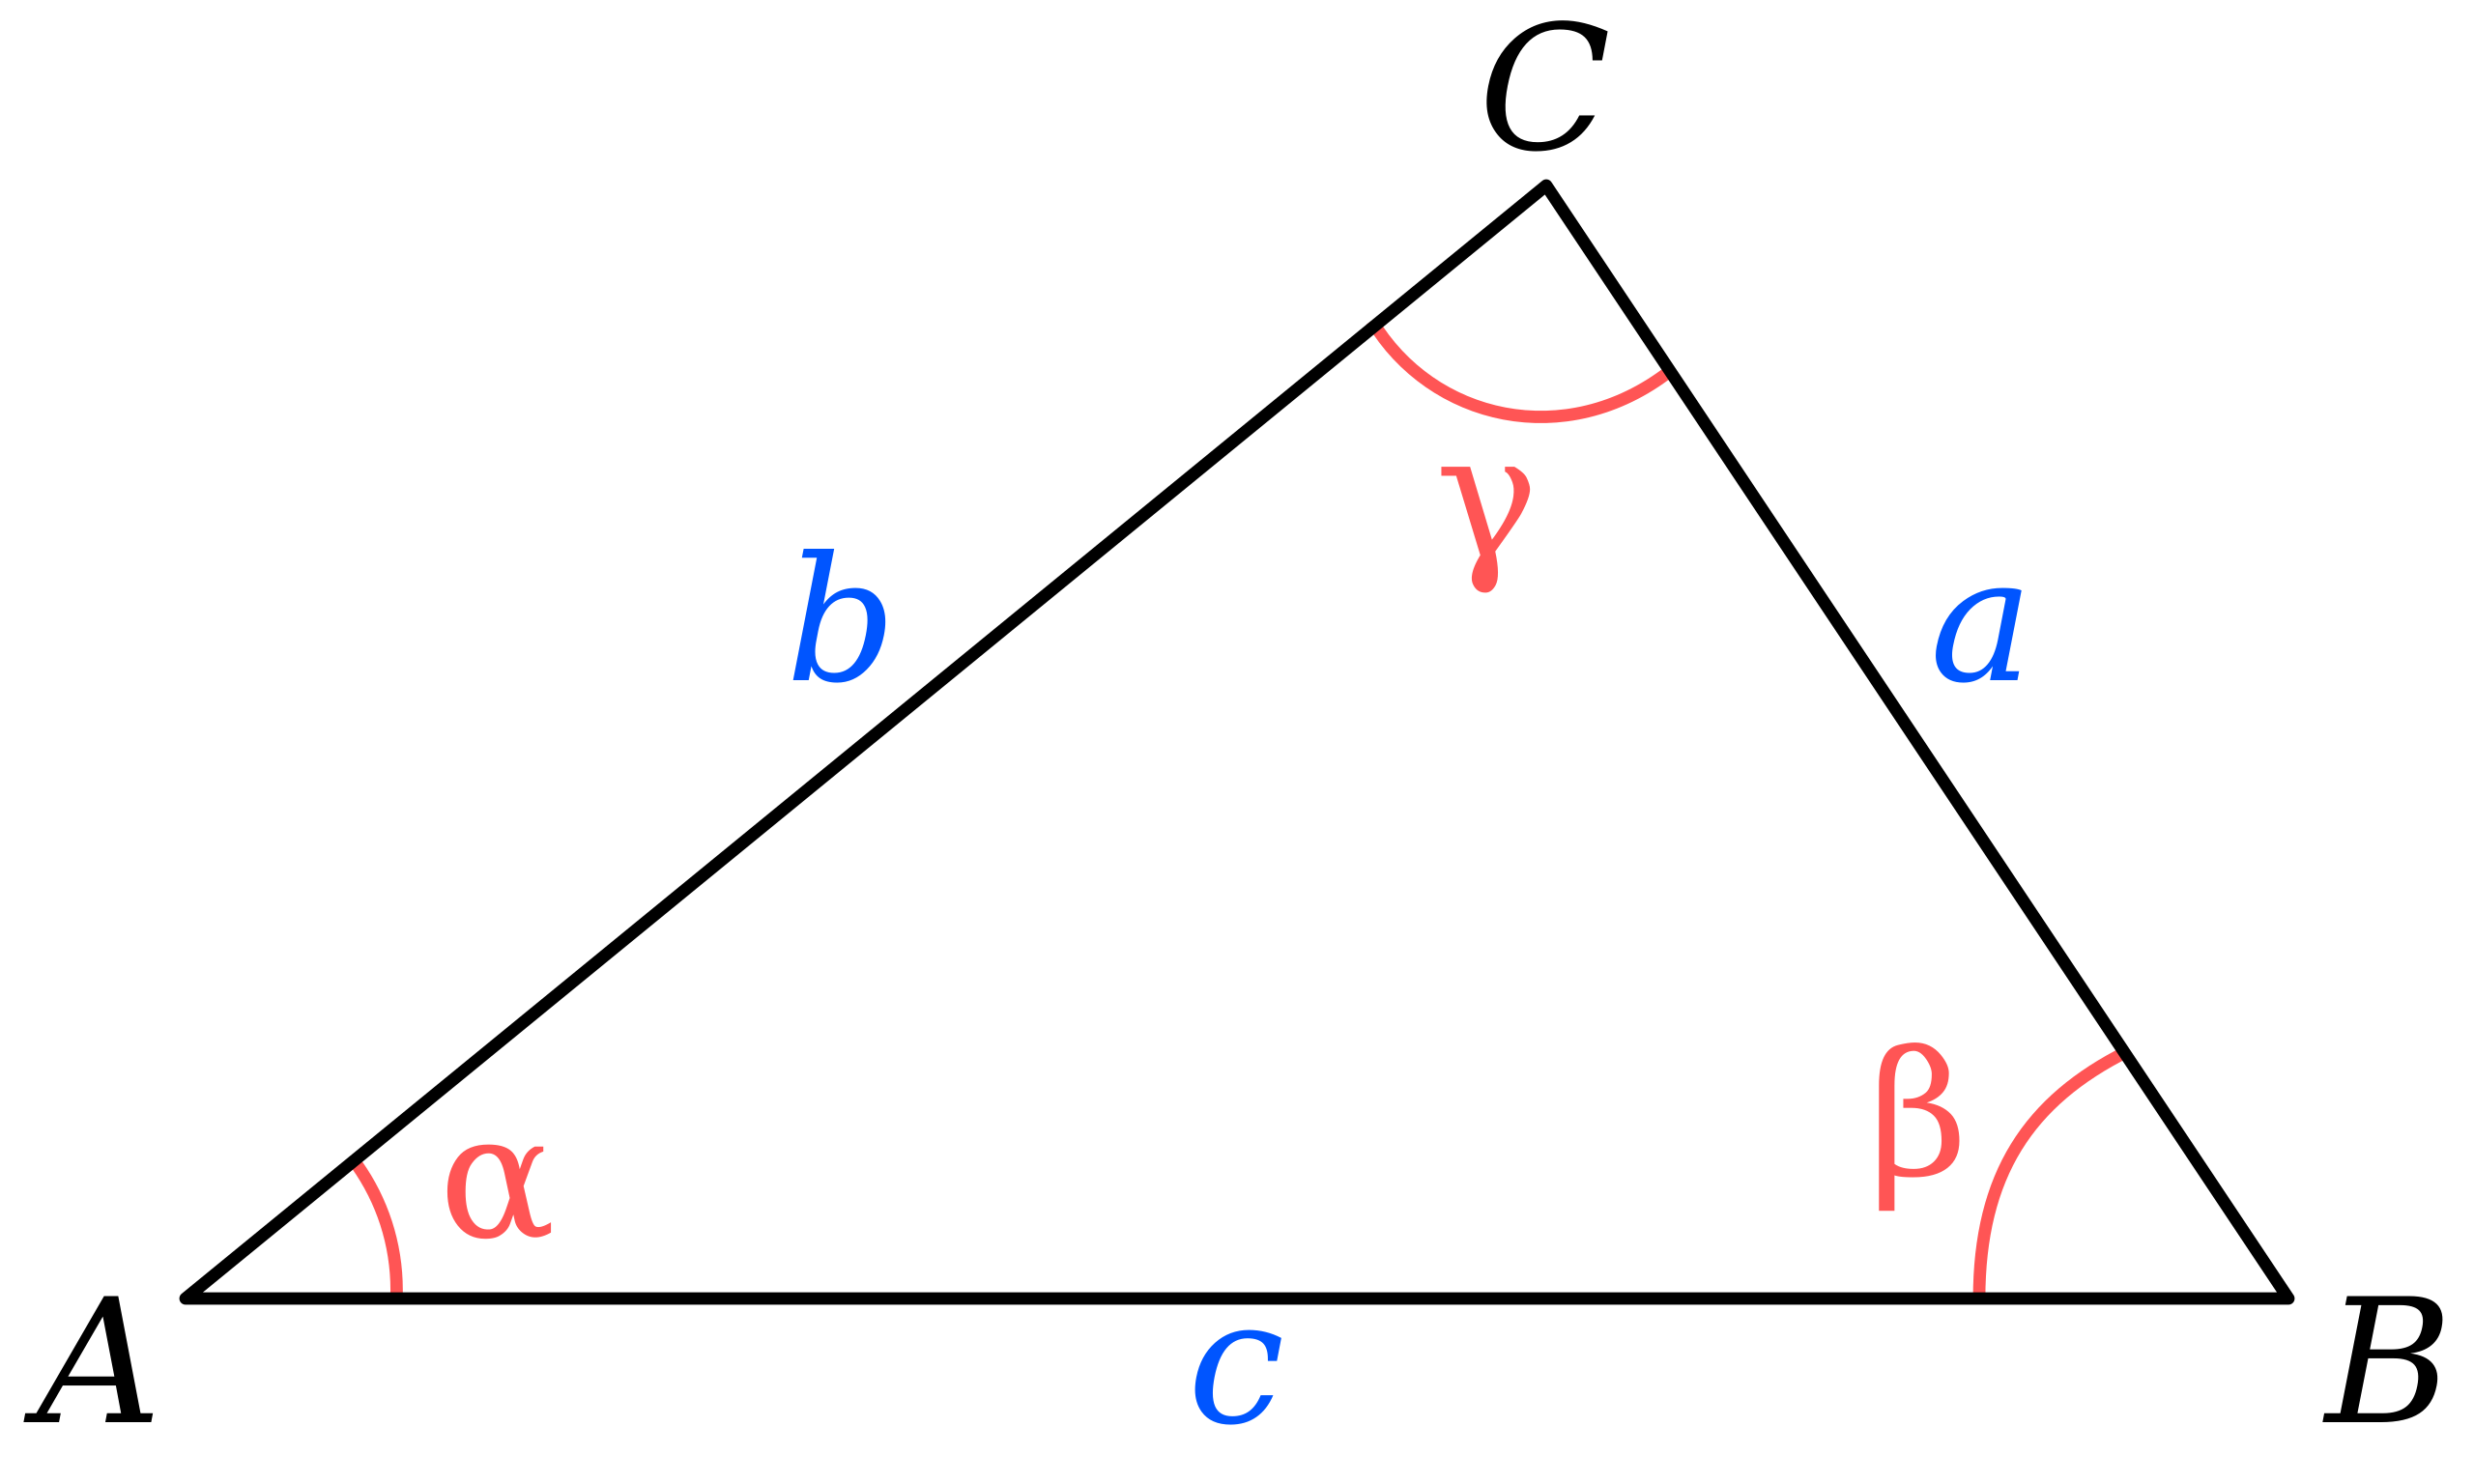
\includegraphics[width=5cm]{cosinediagram.png}
    \caption{Triangle used to illustrate the cosine rule \cite{cosinerulediagram}}
    \label{cosinediag}
    \end{center}
\end{figure}
For the triangle shown in Figure \ref{cosinediag}
\begin{align*}
a^2 &= b^2 + c^2 - 2bc\cos{\alpha}\\
\therefore \cos{\alpha} &= \frac{b^2+c^2-a^2}{2bc}\\
\therefore \alpha &= \arccos{(\frac{b^2+c^2-a^2}{2bc}})
\end{align*}
\paragraph{Calculating Distances}
To calculate real world distances\footnote{Assuming the world is a sphere} from coordinates, Great Circle distance is required. This is the shortest possible distance across the surface of a sphere. The haversine formula\cite{de1795memoria} is one formula that calculates this distance.
For two points $(\phi_1,\lambda_1)$ and $(\phi_2,\lambda_2)$ where $\phi$ and $\lambda$ are latitude and longitude respectively, the great circle distance can be calculated as
\[
d = 2r\arcsin\sqrt{\sin^2{(\frac{\phi_2-\phi_1}{2})}+\cos{\phi_1}\cos{\phi_2}\sin^2{(\frac{\lambda_2-\lambda_1}{2})}}
\]
where $r$ is the radius of the earth, so approximately $6371$ km.
\subsection{Preprocessing and Subsequent Querying of the Graph}
\label{contractiondesign}
There are many different methods of route finding\cite{travelplannervideo}. In the Analysis section I considered both Contraction Hierachies\cite{Geisberger2012} and ALT*. Upon further research, I determined that contraction hierachies would be more
efficient than ALT* in this situation. 
\subsubsection{Contraction Hierachies}
In most road networks there is an inherently hierachical structure. When a human plots a long distance route, they don't consider small dirt tracks, and instead choose the best motorway. 
This is because in most cases motorways are faster. I do not expect the same level of hierachy in figuring out where is cyclable, because cyclists do not have the same limiting factor of the speed limit. However there will still be 
some routes that are obviously the best, at least to my program.\\
\begin{figure}
    \begin{center}
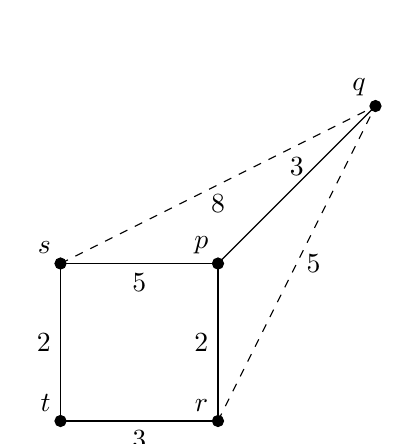
\begin{tikzpicture}
\filldraw (0,0) circle (2pt) node[anchor=south east] {$p$};
\filldraw (2,2) circle (2pt) node[anchor=south east] {$q$};
\filldraw (0,-2) circle (2pt) node[anchor=south east] {$r$};  
\filldraw (-2,0) circle (2pt) node[anchor=south east] {$s$};
\filldraw (-2,-2) circle (2pt) node[anchor=south east] {$t$};
\draw (-2,0) -- (-2,-2) node[pos=0.5,left] {$2$};
\draw (-2,-2) -- (0,-2) node[pos=0.5,below] {$3$};
\draw (-2,0) -- (0,0) node[pos=0.5,below] {$5$};
\draw (0,0) -- (2,2) node[pos=0.5,above] {$3$};
\draw (0,0) -- (0,-2) node[pos=0.5,left] {$2$};
\draw[dashed] (-2,0) -- (2,2) node [pos=0.5,below] {$8$};
\draw[dashed] (0,-2) -- (2,2) node [pos=0.5,right] {$5$};
\end{tikzpicture}
\end{center}
    \caption{The shortcuts that would be added while contracting node $p$}
    \label{Contraction}
\end{figure}
Contraction hierachies work by the process of iterative contraction of nodes. Some order of contraction is defined, in order of least to most important, and the nodes are contracted in this order.
When a node is contracted the shortest paths are calculated between all pairs of neighbour nodes. If the shortest path goes through the node to be contracted a new shortcut is added. This maintains all shortest paths in the Graph. 
An example in an undirected graph is shown in Figure \ref{Contraction}. 
\paragraph{Bidirectional Dijkstra Queries}
The bidirectional variant of dijkstra is a useful speedup technique. A forward search from the source node is interlaced with a backward search from the target node. When a node is settled by both searches all nodes on the shortest path are known to have been settled.
This variant can reduce the search space, and ideas from this search are used when querying the contracted graph.
\paragraph{Querying the Contracted Graph}
When contraction is complete, a new graph is created called G*. This Graph contains all of the nodes and edges in the original graph, as well as all of the shortcuts created during the contraction process.
All nodes have a new item of information attached to them, known as the hierachy. The first node to be contracted will have a hierachy of 1, and the last node to be contracted will have a hierachy of $n$. 
Two new graphs can be developed from the hierachy:
$G*\uparrow$ and $G*\downarrow$. $G*\uparrow$ contains only edges where the hierachy increases, and $G*\downarrow$ contains the opposite. In order to find the shortest path between two nodes $u$ and $v$, a bidirectional search
 consisting of a forward search in $G*\uparrow$ and a backward search in $G*\downarrow$. In an undirected graph this is the same as two forward searches in $G*\uparrow$, but in a directed graph the backwards search must go backwards on directed edges.
Implementing this will require the \texttt{GeographicNode} equivalent class in \texttt{ContractableGraph} to contain incoming connections and shortcuts. It has been proven\cite{Geisberger2012} that this method of query will leave at least one node on the shortest path settled by both the forward and backward searches.
\paragraph{Finding the shortest route}
Once the query is completed, a node on the shortest path will be in the intersection of both searches. The total distance of a route containing a given node is the sum of the distance from the forward search and the distance from the backward search. So to find a node on the shortest path,
the minimum total distance cost in the intersection of both searches must be found. From there the \texttt{prev} values can be used to backtrack to the start and end of the route. At this point the route will almost certainly contain shortcuts, which must be somehow expanded into their original form.
\paragraph{Limitations}
When using contraction hierachies, turn costs cannot be as easily integrated because the cost function must be per edge not for collections of edges. It is possible to use a second graph which has the original graph's edges as nodes, but this approach would slow down contraction, and add more complexity to the project.
Therefore the ability to consider turn costs will only be added to the simple dijkstra searches and any turn costs will be ignored in the preprocessing mode.
\paragraph{Node Order}
The optimal node ordering is the one that minimises the expected query time. This can be estimated to be the same as the ordering that leads to the lowest total amount of shortcuts being added, which will in turn minimise the expected search space size.
Finding the best ordering is an NP-hard problem, as it requires simulating every possible node ordering to find which one gives the best results. Instead the contraction algorithm will use a heuristic based approach. There are many heuristics of varying complexity, but the 
two that my design uses are the difference between the amount of shortcuts added and edges removed, and the number of deleted neighbours. Keeping the number of deleted neighbours low makes sure the contraction is spread out across the graph. When contraction is not uniform, very poor performance is attained.
The edge difference is essentially a metric of how simple the graph would be after the contraction, so it makes sense to greedily make the graph as simple as possible. The edge difference heuristic can be calculated by simulating the contraction of a node.
The deleted neighbours heuristic can only go up as the graph is contracted, and the same tends to happen for the difference of edges. Therefore it makes sense to load all of the nodes into a priority queue by their heuristic values,
and pull out the minimum node. If the heuristic value has changed since the heuristic was placed into the priority queue the node is reinserted into the queue with the new value, otherwise it is contracted.    
\paragraph{Optimising Contraction}
In order to contract a node, and compute the edge difference, it needs to be ascertained which pairs of neighbour nodes have their shortest path going through the node. If checking individually for each pair, there would be $O(n^2)$ queries.
Instead a variant of dijkstra's algorithm can be used, with a stopping condition of settling all the other neighbour nodes instead of just one. These queries might take slightly longer, but they would find all $n$ neighbour nodes.
Another useful optimisation technique is to refill the priority queue every so often, for instance when lots of re-insertions have to happen. 
\subsection{Saving the work done to disk}
\label{sec:serialization}
So that intensive workloads such as contracting the graph do not need to be repeated a facility for saving and loading this information must exist.
It would be possible to write some manual serialisation code, but it is simpler to just save the whole class objects. Kotlin has a 
fairly easy to use serialisation library that can serialise whole objects to disk\cite{kotlinh}. The standard mode for this is serialising to JSON, but as my files will likely be very large, my design uses the alternate CBOR encoding instead.
As mentioned previously, \texttt{GeographicNode} objects cannot contain other \texttt{GeographicNode} objects. This is because the kotlin serialiser will get stuck recursively serialising the same nodes. 
CBOR\footnote{Concise Binary Object Representation} can be used for more consise binary representation of JSON objects.
\subsection{User Interface}
My design calls for a simple terminal based user interface. Users should be able to load maps and preprocessed data from pre existing files, and trigger addtional preprocessing at different levels. This can be simply implemented by means of a loop where users can choose options or end the program.
\subsection{Route Output}
In order to fulfil specification point \ref{followpossible}, the route must be output in a format that is not just a list of coordinates. Writing software that can use a route to give turn by turn directions, 
along with route recalculation when straying off the route is beyond the bounds of this project. However such software does already exist. One example of this is Osmand, an application that uses Open Street Map data to provide a routing application.
Osmand can generate it's own routes, but it can also be used to follow routes stored in gpx files. GPX files are a subset of XML that can be used to store geographic data such as routes. Many other applications accept these, so a user would not 
be limited to Osmand. Writing to a GPX file manually would be boring, so my design calls for the use of a library. 
\section{Data Structure Overview}
\newpage
\chapter{Technical Implementation}
\section{Overview}
\begin{figure}[p]
\begin{verbatim}
$ tree
.
├── accidents
│   ├── 2005.json
│   ├── 2006.json
│   ├── 2007.json
│   ├── 2008.json
│   ├── 2009.json
│   ├── 2010.json
│   ├── 2011.json
│   ├── 2012.json
│   ├── 2013.json
│   ├── 2014.json
│   ├── 2015.json
│   ├── 2016.json
│   ├── 2017.json
│   ├── 2018.json
│   └── 2019.json
├── build.gradle.kts
├── download.py
├── gradlew
├── gradlew.bat
├── maps
│   ├── course_m25_boundary.json
│   ├── cyclable.osm
│   ├── cyclable.osm.pbf
│   ├── goldhawk.osm
│   ├── testarea.json
│   ├── testarea.osm
│   └── ways.osm
├── output.json
├── parse.py
├── display.py
├── route.gpx
├── savedGraph.bin
├── settings.gradle.kts
└── src
   └── main
        └── kotlin
            ├── ContractableGraph.kt
            ├── ContractableGraphTest.kt
            ├── DoubleTuple.kt
            ├── GeographicGraph.kt
            ├── GeographicGraphTest.kt
            ├── IntTuple.kt
            ├── Main.kt
            ├── MainKtTest.kt
            ├── OpenStreetMap.kt
            └── OpenStreetMapTest.kt
6 directories, 42 files
\end{verbatim}
\caption{Project file structure. Automatically generated files have been omitted}
\label{fsystem}
\end{figure}
Figure \ref{fsystem} shows the complete file system. The \texttt{accidents} subfolder is used to generate \texttt{output.json}, and the \texttt{maps} folder contains different \texttt{osm} files for 
different areas. All of the \texttt{.py} files are used in the creation of \texttt{output.json} and all of the files in \texttt{src/main/kotlin} are make up the program as a whole, with \texttt{Main.kt} as the entry point.
\section{Accident Download System}
\label{Accident Download System Implementation}
As this system only really needs to be run once, I just wrote some hacky python scripts to do this.
As mentioned in Section \ref{Pulling from the TFL API}, I used a simple script called \texttt{download.py} to pull all the relevant accident data from the TFL API and store it in the \texttt{accidents} folder.
\begin{lstlisting}[language=python]
import requests
import json
for year in range(2005,2020):
    print(year)
    response = requests.get(f"https://api.tfl.gov.uk/AccidentStats/{year}")
    with open(f"accidents/{year}.json","w") as yearfile:
        json.dump(response.json(),yearfile)
\end{lstlisting}
In order to extract useful information from these files, I used \texttt{parse.py} to extract all those accidents where one of the listed casulaties was a cyclist. While data exists between 2005 and 2019,
when looking at some of the areas with high accident density, I found that the accident density had greatly decreased in recent years. This led to the realisation that the TFL accident data was not solely collected 
for the purpose of providing interesting data for A-Level NEA coursework, and that TFL was probably looking at the data as well and fixing those areas which were lethal. Thus I decided to only use accidents from after 2010.
\begin{lstlisting}[language=python]
import json
#we want to parse for accidents that happened to cyclists and store the severity and the location
accidents = []
for year in range(2010,2020):
    print(len(accidents), year)
    with open(f"accidents/{year}.json","r") as outfile:
        data = json.load(outfile)
    for x in data:
        try:
            if x["casualties"]["mode"] == "PedalCycle":
                accidents.append([x["lat"],x["lon"],x["severity"]])
        except:
            if len([person for person in x["casualties"] if person["mode"] == "PedalCycle"]) >= 1:
                accidents.append([x["lat"],x["lon"],x["severity"]])
with open("output.json","w") as outfile:
    json.dump(accidents,outfile)
\end{lstlisting}
I also wrote a small visualisation script using matplotlib to verify that the data was dense enough to be useful and imported correctly. I called this \texttt{display.py}. 
\begin{lstlisting}[language=python]
import json
import matplotlib.pyplot as plt
x = []
y = []
with open("output.json","r") as inputfile:
    data = json.load(inputfile)
for accident in data:
    x.append(accident[1])
    y.append(accident[0])
    print(accident[0],accident[1])
plt.scatter(x,y,0.05)
plt.show()
\end{lstlisting}
\begin{figure}[h]
    \begin{center}
    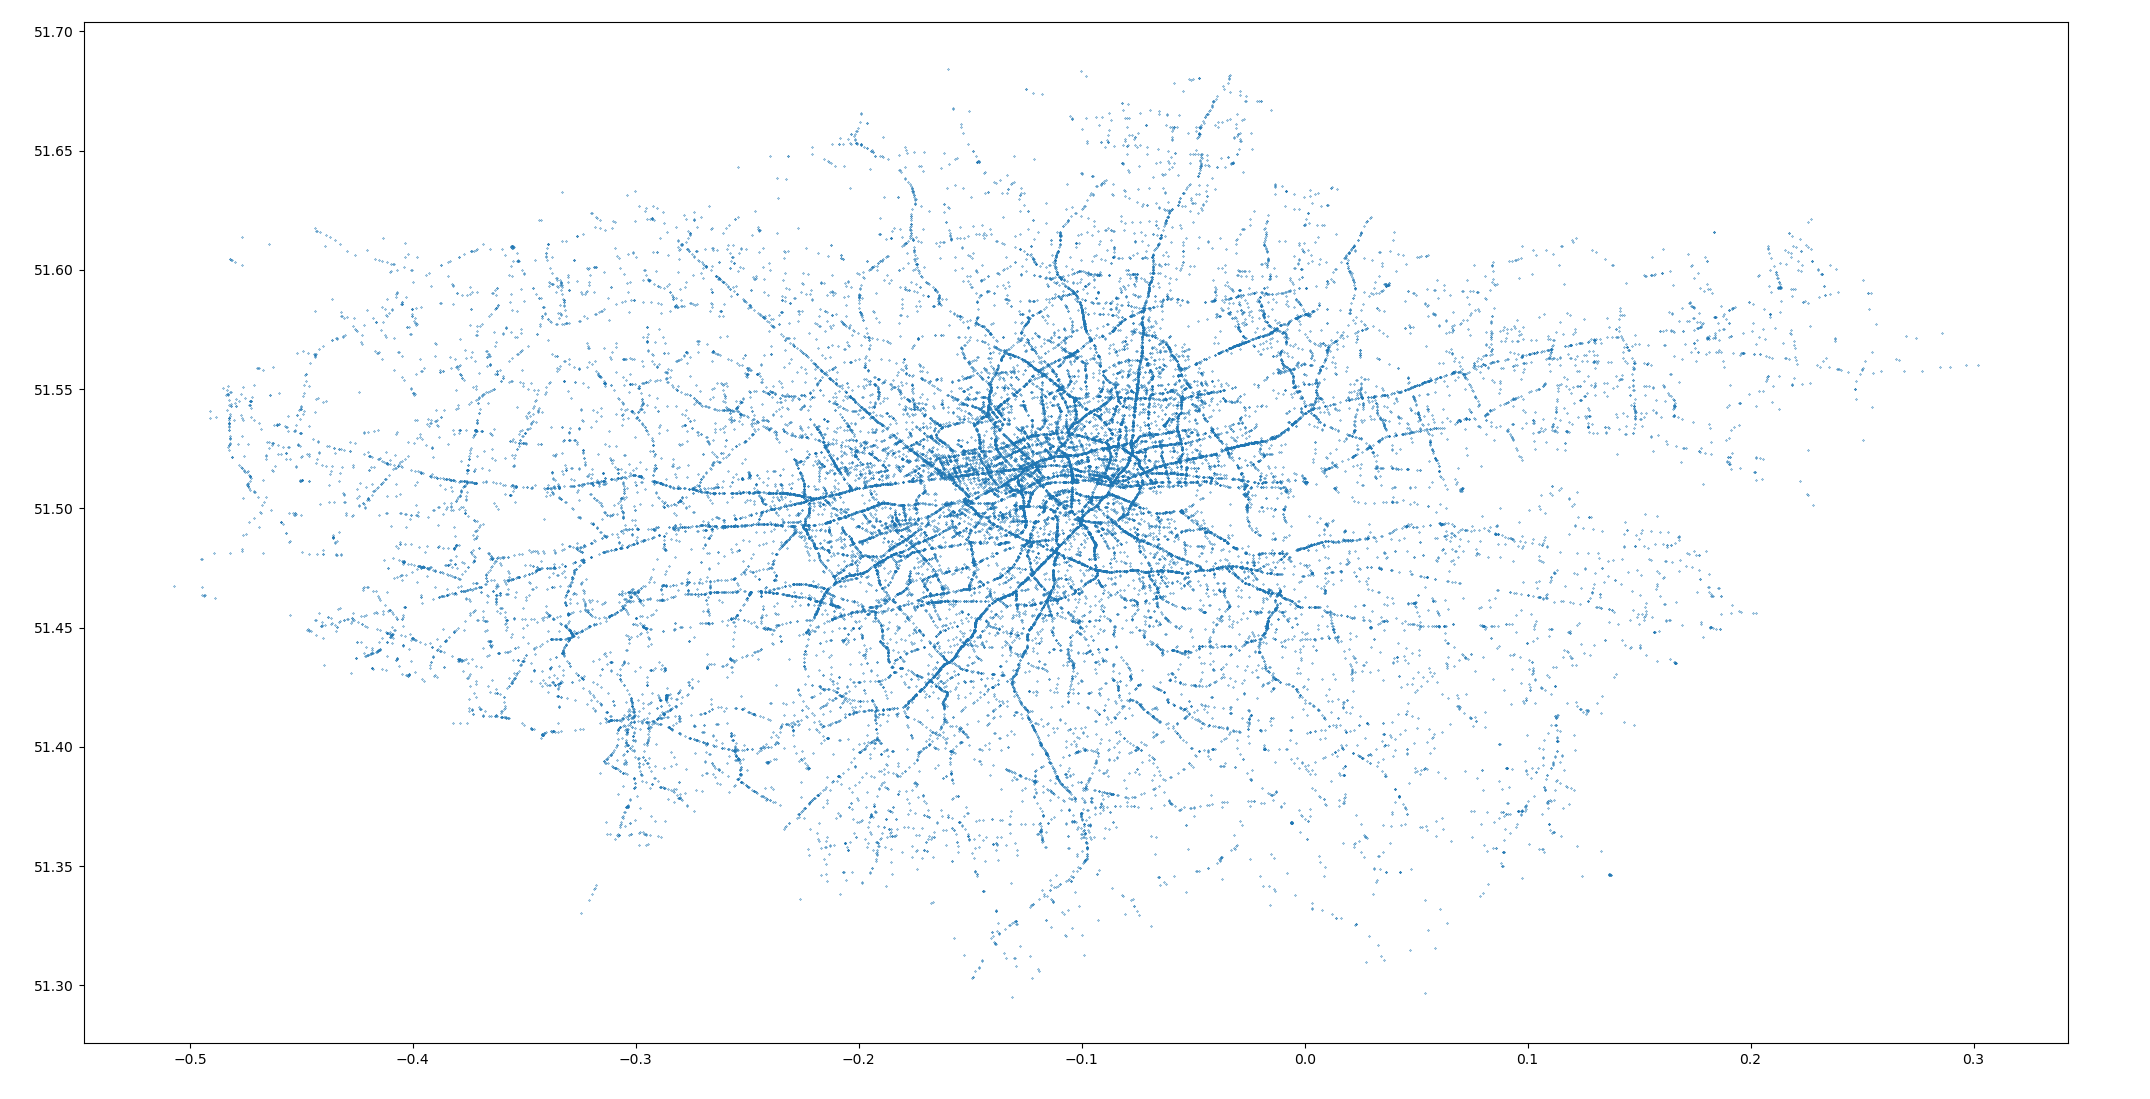
\includegraphics[width=18cm]{chart.png}
    \end{center}
    \caption{Plot of all accidents in which there were injured cyclists in London since 2010}
    \label{chart}
\end{figure}
This generated the plot shown in Figure \ref{chart}. Major roads are clearly visible, so a route finding algorithm will be able to avoid these. One problem that was apparent from the data was that there 
are significantly more accidents in central London then in the suburbs. Central London may be more dangerous, but there are also far more cyclists, and as I cannot get road usage data easily routes will probably be biased against
central london, possibly causing them to go around. Hopefully, the distance cost will pull routes back towards central London, and they will instead pick between roads for safety on a more local level.
\newpage
\section{Route Finding System}
\begin{figure}
    \begin{center}
        \includegraphics[width=10cm]{finaluml.png}
    \end{center}
    \caption{Final Project UML Diagram}
    \label{finaluml}
\end{figure}
The accident download system of the previous section only really serves to provide the input for this system. This system \textit{is the project}. Figure \ref{finaluml} shows the completed UML diagram. \texttt{IntTuple} and \texttt{DoubleTuple}, which are used in priority queues,  have been added since the class hierachy was designed but overall the structure has remained the same.
\subsection{Parsing Open Street Map Data}
The \texttt{OpenStreetMap} class contains the methods for parsing \texttt{.osm} files and forming a new \texttt{GeographicGraph} class. Some of these methods cannot be called in the init method of \texttt{GeographicGraph} because 
they operate on the graph after it has been populated by \texttt{parseXML}, so they are placed in the constructor for \texttt{OpenStreetMap}. This constructor calls \texttt{parseXML}.
\begin{lstlisting}[language=kotlin]
private fun parseXML(filename: String) {
    val stream = File(filename).inputStream()
    val saxReader = SAXReader()
    val cyclableDocument = saxReader.read(stream)
    val root: Element = cyclableDocument.rootElement
    val it: Iterator<Element> = root.elementIterator()
    while (it.hasNext()) {
        val element: Element = it.next()
        when (element.qName.name) {
            "node" -> processNode(element)
            "way" -> processWay(element)
        }
    }
}
\end{lstlisting}
All that \texttt{parseXML} does is iterate through all of the subelements in the input xml file, then calls either \texttt{processNode} or \texttt{processWay}. The \texttt{processNode} function just adds all nodes it sees to the \texttt{cyclableGraph}, and the real logic is dealt with in \texttt{processWay}.
\begin{lstlisting}[language=kotlin]
private fun processWay(way: Element) {
    var oneWay = false
    var cycleWay = false
    var slowWay = false
    val nodes = mutableListOf<Long>()
    val acceptedRoads = mutableListOf(
        "bridleway",
        "trunk",
        "pedestrian",
        "service",
        "primary",
        "secondary",
        "tertiary",
        "unclassified",
        "residential",
        "primary_link",
        "secondary_link",
        "tertiary_link",
        "living_street",
        "cycleway",
        "footway"
    )
    val disallowedSurfaces = mutableListOf("unpaved", "fine_gravel", "gravel", "dirt", "grass", "pebblestone")
    val disallowedAccess = mutableListOf("no")
    val highSpeed = mutableListOf("40 mph", "50 mph", "60 mph", "70 mph")
    val tags = HashMap<String, String>()
    val it = way.elementIterator()
    while (it.hasNext()) {
        val subElement = it.next()
        if (subElement.qName.name == "nd") {
            nodes.add(subElement.attribute("ref").value.toLong())
        }
        if (subElement.qName.name == "tag") {
            tags[subElement.attributeValue("k")] = subElement.attributeValue("v")
        }
    }
    val highwayType = tags["highway"].toString()
    val access = tags["access"].toString()
    val surface = tags["surface"].toString()
    val note = tags["note"].toString()
    val bicycle = tags["bicycle"].toString()
    val oneway = tags["oneway"].toString()
    val maxspeed = tags["maxspeed"].toString()
    val towpath = tags["towpath"].toString()
    val motor = tags["motor_vehicle"].toString()
    if (!acceptedRoads.contains(highwayType)) return
    if (highSpeed.contains(maxspeed)) return
    if (oneway == "yes") oneWay = true
    if (highwayType == "cycleway") cycleWay = true
    if (highwayType == "footway") {
        cycleWay = true
        slowWay = true
    }
    if (highwayType == "pedestrian") {
        cycleWay = true
        if (bicycle != "designated") {
            slowWay = true
            }
    }
    if (note == "towpath") return
    if (disallowedAccess.contains(access) && bicycle != "yes") return
    if (disallowedAccess.contains(bicycle)) return
    if (disallowedSurfaces.contains(surface)) return
    if (!acceptedRoads.contains(highwayType)) return
    if (towpath == "yes") return
    if (motor == "private") cycleWay = true
    if (cycleWay) {
        cyclableGraph.safeNodes.addAll(nodes)
    }
    if (slowWay) {
        cyclableGraph.slowNodes.addAll(nodes)
    }
    for (i in 1 until nodes.size) {
        cyclableGraph.addEdge(nodes[i - 1], nodes[i], oneWay)
    }
}
\end{lstlisting}
All of the relevant values from \texttt{tags} are converted to string in order to eliminate the need for any null checks. If a way doesn't have a certain tag the value will be \texttt{"null"}, which is of course not in any of the allow or disallow lists.
If the way is determined to be "safe" or "slow", all the nodes in the way are added to the relevant set in \texttt{cyclableGraph}. 
\section{Graph Representation}
As shown in Figure \ref{finaluml}, the \texttt{GeographicGraph} class is used to represent London. This is through the \texttt{GeographicNode} inner class, which stores both incoming and outgoing connections as well as the weight of the node. 
\subsubsection{Graph Setup}
Once all the nodes and connections have been added and the \texttt{safeNodes} and \texttt{slowNodes} sets have been filled up by the parsing functions in \texttt{OpenStreetMap}, some other functions need to be run to set up the graph for operations and otherwise clean up.
These functions are called from the intialisation method of \texttt{OpenStreetMap}. 
\paragraph{Graph Pruning}
The first function called is \texttt{pruneDisconnected}. This function ensures that the graph is strongly connected by finding the largest strongly connected component and deleting all nodes not in it. This ensures that the program can easily 
conform to Specification Point \ref{nocrashy}, as it ensures that it is possible to find a route between any two points in the graph. 
\begin{lstlisting}[language=kotlin]
fun pruneDisconnected() {
    fun getPostOrderTraversal(vertice : Long, visited : HashSet<Long>, getNeighbours : (Long) -> HashSet<Long>): List<Long> {
        var searchStack = Stack<Long>()
        var postOrder = LinkedList<Long>()
        searchStack.add(vertice)
        while (searchStack.size != 0)
        {
            var current = searchStack.pop()
            if (!visited.contains(current))
            {
                visited.add(current)
                postOrder.add(current)
                for (neighbour in getNeighbours(current))
                {
                    searchStack.push(neighbour)
                }
            }
        }
        return postOrderStack
    }
    var visited = HashSet<Long>()
    val L = LinkedList<Long>()
    for (vertice in vertices)
    {
        for (item in getPostOrderTraversal(vertice.key,visited) { id -> vertices[id]!!.connections })
        {
            L.addFirst(item)
        }
    }
    visited = HashSet<Long>()
    val components = HashMap<Long, HashSet<Long>>()
    for (vertice in L)
    {
        var postOrder = getPostOrderTraversal(vertice,visited) { id -> vertices[id]!!.incomingConnections }
        if (postOrder.size != 0)
        {
            components[vertice] = HashSet<Long>()
            for (item in postOrder)
            {
                components[vertice]?.add(item)
            }
        }
    }
    val mainComponent = components.maxByOrNull { component -> component.value.size }!!
    val before = vertices.size
    vertices = vertices.filter { item -> mainComponent.value.contains(item.key) } as HashMap<Long, GeographicNode>
    val after = vertices.size
    println("Shrunk vertices from $before to $after")
    for (vertice in vertices.values)
    {
        vertice.connections = vertice.connections.filter { id -> vertices.containsKey(id) }.toHashSet()
        vertice.incomingConnections = vertice.incomingConnections.filter { id -> vertices.containsKey(id)}.toHashSet()
    }
}
\end{lstlisting}
I had to slightly modify Kosaraju's Algorithm\cite{wikipedia_2022}, as it called for the use of recursive functions. As the strongly connected component that my program uses to represent London has more than a million nodes, any recursive
solution was clearly going to run out of stack depth or stack space. Therefore I modified it to use a iterative approach, using the stack \texttt{searchStack}, and the list \texttt{postOrder}.\\ In order to avoid rewriting the subfunction \texttt{getPostOrderTraversal} for the case in which the search is performed backwards, I passed in a lambda function that is used to find either outgoing or incoming neighbours. 
Once all the strongly connected components are placed in the HashMap \texttt{components}, the largest one can be quickly ascertained. From there, all that is required is the actual pruning of the process.
First, the \texttt{vertices} are filtered for nodes that are in the largest strongly connected component, then all of these vertices have their connections filtered to ensure that traversal algorithms do not attempt to lookup vertices which no longer exist.
\paragraph{Setting up the R*Tree}
As discussed in Section \ref{Rtree}, I used an R*Tree to facilitate fast lookup of nodes from nearby coordinates. The library I used\cite{rtree} supports both iterative loading of the rtree and bulk loading. Bulk loading is faster and can result in a 
more efficient R*Tree, so \texttt{setupRTree} uses that. The R*Tree generated is visualised in Figure \ref{rvis}.
\begin{figure}[t]
\begin{center}
    \includegraphics[width=10cm]{rtree.png}
\end{center}
\caption{The RTree containing all of the OSM nodes in London}
\label{rvis}
\end{figure}
\begin{lstlisting}[language=kotlin]
fun setupRTree() {
    if (nodeTree.size() != 0) {
        return
    }
    var nodeList = mutableListOf<Entry<Long, Geometry>>()
    for (node in vertices) {
        nodeList.add(Entries.entry(node.key, Geometries.point(node.value.longitude, node.value.latitude)))
    }
    nodeTree = RTree.star().maxChildren(28).create(nodeList)
}
\end{lstlisting}
The function also includes a safety check to make sure that the R*Tree has not been loaded before, as if it had the entries would be added twice. 
\newpage
\paragraph{Gathering Weights}
This system simply reads the output from the Accident Download System, and attaches weights to the nearest node to every accident. I decided on the arbitrary scoring system of 1 point for Slight accidents, 2 points for Severe accidents, and 3 points for Fatal accidents. 
\begin{lstlisting}[language=kotlin]
fun gatherWeights() {
    val accidentFile = File("output.json")
    val accidents = JSONArray(accidentFile.inputStream().readBytes().toString(Charsets.UTF_8))
    for (accident in accidents) {
        val parsedAccident = accident as JSONArray
        val latitude: Double = (parsedAccident[0] as BigDecimal).toDouble()
        val longitude: Double = (parsedAccident[1] as BigDecimal).toDouble()
        val severity = parsedAccident[2] as String
        try {
            val additionNode = vertices[getNearestNode(latitude, longitude)]!!
            when (severity) {
                "Slight" -> additionNode.weight += 1
                "Severe" -> additionNode.weight += 2
                "Fatal" -> additionNode.weight += 3
            }
        } catch (e: InvalidParameterException) {
            //In this case we can still apply all the other accidents, even if this accident doesn't match well.
            continue
        }
    }
}
\end{lstlisting}
In order to find the nearest node, this function calls another function called \texttt{getNearestNode}. This is shown below.
\begin{lstlisting}[language=kotlin]
private fun getNearestNode(latitude: Double, longitude: Double): Long {
    val closestNodeObserver = nodeTree.nearest(Geometries.point(longitude, latitude), 0.005, 1)
    try {
        val closestNode = closestNodeObserver.first()
        return closestNode.value()
    } catch (e: NoSuchElementException) {
        //If this happens the coordinates are very far from the nearest node, so a appropriate node cannot be found.
        //Therefore an error should be thrown
        throw InvalidParameterException()
    }
}
\end{lstlisting}
The \texttt{InvalidParameterException} is thrown by \texttt{getNearestNode} if there is no node within 0.005 degrees. This is roughly half a kilometer, so all reasonable ranges of nodes can be found. Selecting a smaller value for
 the maximum search distance makes the query faster. In \texttt{gatherWeights} this can be safely ignored as while a few coordinates might be too far away from nodes the vast majority will not be.\\
Finally, all known safe nodes have their weights set to 0. This completes the graph setup.
\subsubsection{Graph Queries}
\texttt{GeographicGraph} has 3 main methods that will be queried by the user facing code. These are \texttt{getRandomId}, \texttt{getNearestNode}, and \texttt{findRoute}. \texttt{getRandomId} just returns a random vertice id from the vertices HashMap, and \texttt{getNearestNode} has already been explained.
\texttt{findRoute} provides functionality for deciding which route finding method to use, then executing it. In my design I allowed only one instance of \texttt{contractedGraph}, but when implementing I decided to change this to allow as many contractions as wanted. This was implemented through a HashMap that holds all the instances of \texttt{contractedGraph}, which are used to find routes when matching parameters are given. 
So the \texttt{findRoute} function calls the corresponding function in the preprocessed graph, or the private function \texttt{findRouteNonContracted}. This is shown below.
\begin{lstlisting}[language=kotlin]
/**
* Basic dijkstra
*/
private fun calculateRoute(
    start: Long,
    end: Long,
    accidentsPerKilometre: Double,
    accidentsPerTurn: Double
): Pair<MutableList<Long>, Double> {
    val F = PriorityQueue<DoubleTuple>()
    val dist = HashMap<Long, Double>()
    val prev = HashMap<Long, Long>()
    dist[start] = 0.0
    prev[start] = -1
    var u: Long
    val toAdd = DoubleTuple(start, 0.0)
    F.add(toAdd)
    while (F.size != 0) {
        val item = F.poll()
        u = item.id
        if (dist[u] != item.dist) continue
        if (u == end) {
            return Pair(solution(end, prev), dist[end]!!)
        }
        for (neighbour in vertices[u]?.connections!!) {
            var alt = dist[u]?.plus(vertices[neighbour]?.weight!!)
            alt = alt?.plus(getDistanceCost(u, neighbour) * accidentsPerKilometre)
            alt = alt?.plus(getTurnCost(prev[u]!!, u, neighbour, accidentsPerTurn))
            if (alt != null) {
                if (!dist.containsKey(neighbour) || alt < dist[neighbour]!!) {
                    dist[neighbour] = alt
                    prev[neighbour] = u
                    val toAdd = DoubleTuple(neighbour, dist[neighbour]!!)
                    F.add(toAdd)
                }
            }
        }
    }
    throw InvalidParameterException()
}

fun findRouteNonContracted(
    start: Long,
    end: Long,
    accidentsPerKilometre: Double,
    accidentsPerTurn: Double
): MutableList<Long> {
    return calculateRoute(start, end, accidentsPerKilometre, accidentsPerTurn).first
}

fun solution(end: Long, prev: HashMap<Long, Long>): MutableList<Long> {
    val route = mutableListOf<Long>()
    var current = end
    while (current.toInt() != -1) {
        route.add(current)
        current = prev[current]!!
    }
    return route.asReversed()
}
\end{lstlisting}
The notable difference between this code and what was designed is that when a tentative distance is updated the old value in the priority queue is not removed. This is because removing items from the middle of priority queues can be quite expensive,
and it is actually cheaper just to leave it in there and just ignore it when eventually polled.\\
The \texttt{DoubleTuple} class is used to allow nodes weights in the priority queue to be based on their distance from the start node rather than the value of the node. The \texttt{DoubleTuple} class implements \texttt{Comparable}, 
so that it can be compared to other \texttt{DoubleTuple} objects by the distance. This allows the tuples to be packed into the priority queue with a weighting based on distance.
\begin{lstlisting}[language=kotlin]
class DoubleTuple(val id : Long, val dist : Double) : Comparable<DoubleTuple>
{
    override fun compareTo(other: DoubleTuple): Int {
        if(dist > other.dist)
        {
            return 1
        }
        else if(dist == other.dist)
        {
            return 0
        }
        else
        {
            return -1
        }
    }
 }
\end{lstlisting}
\newpage
\section{Graph Contraction and Querying}
\subsubsection{Graph Contraction}
\begin{figure}[t]
\begin{center}
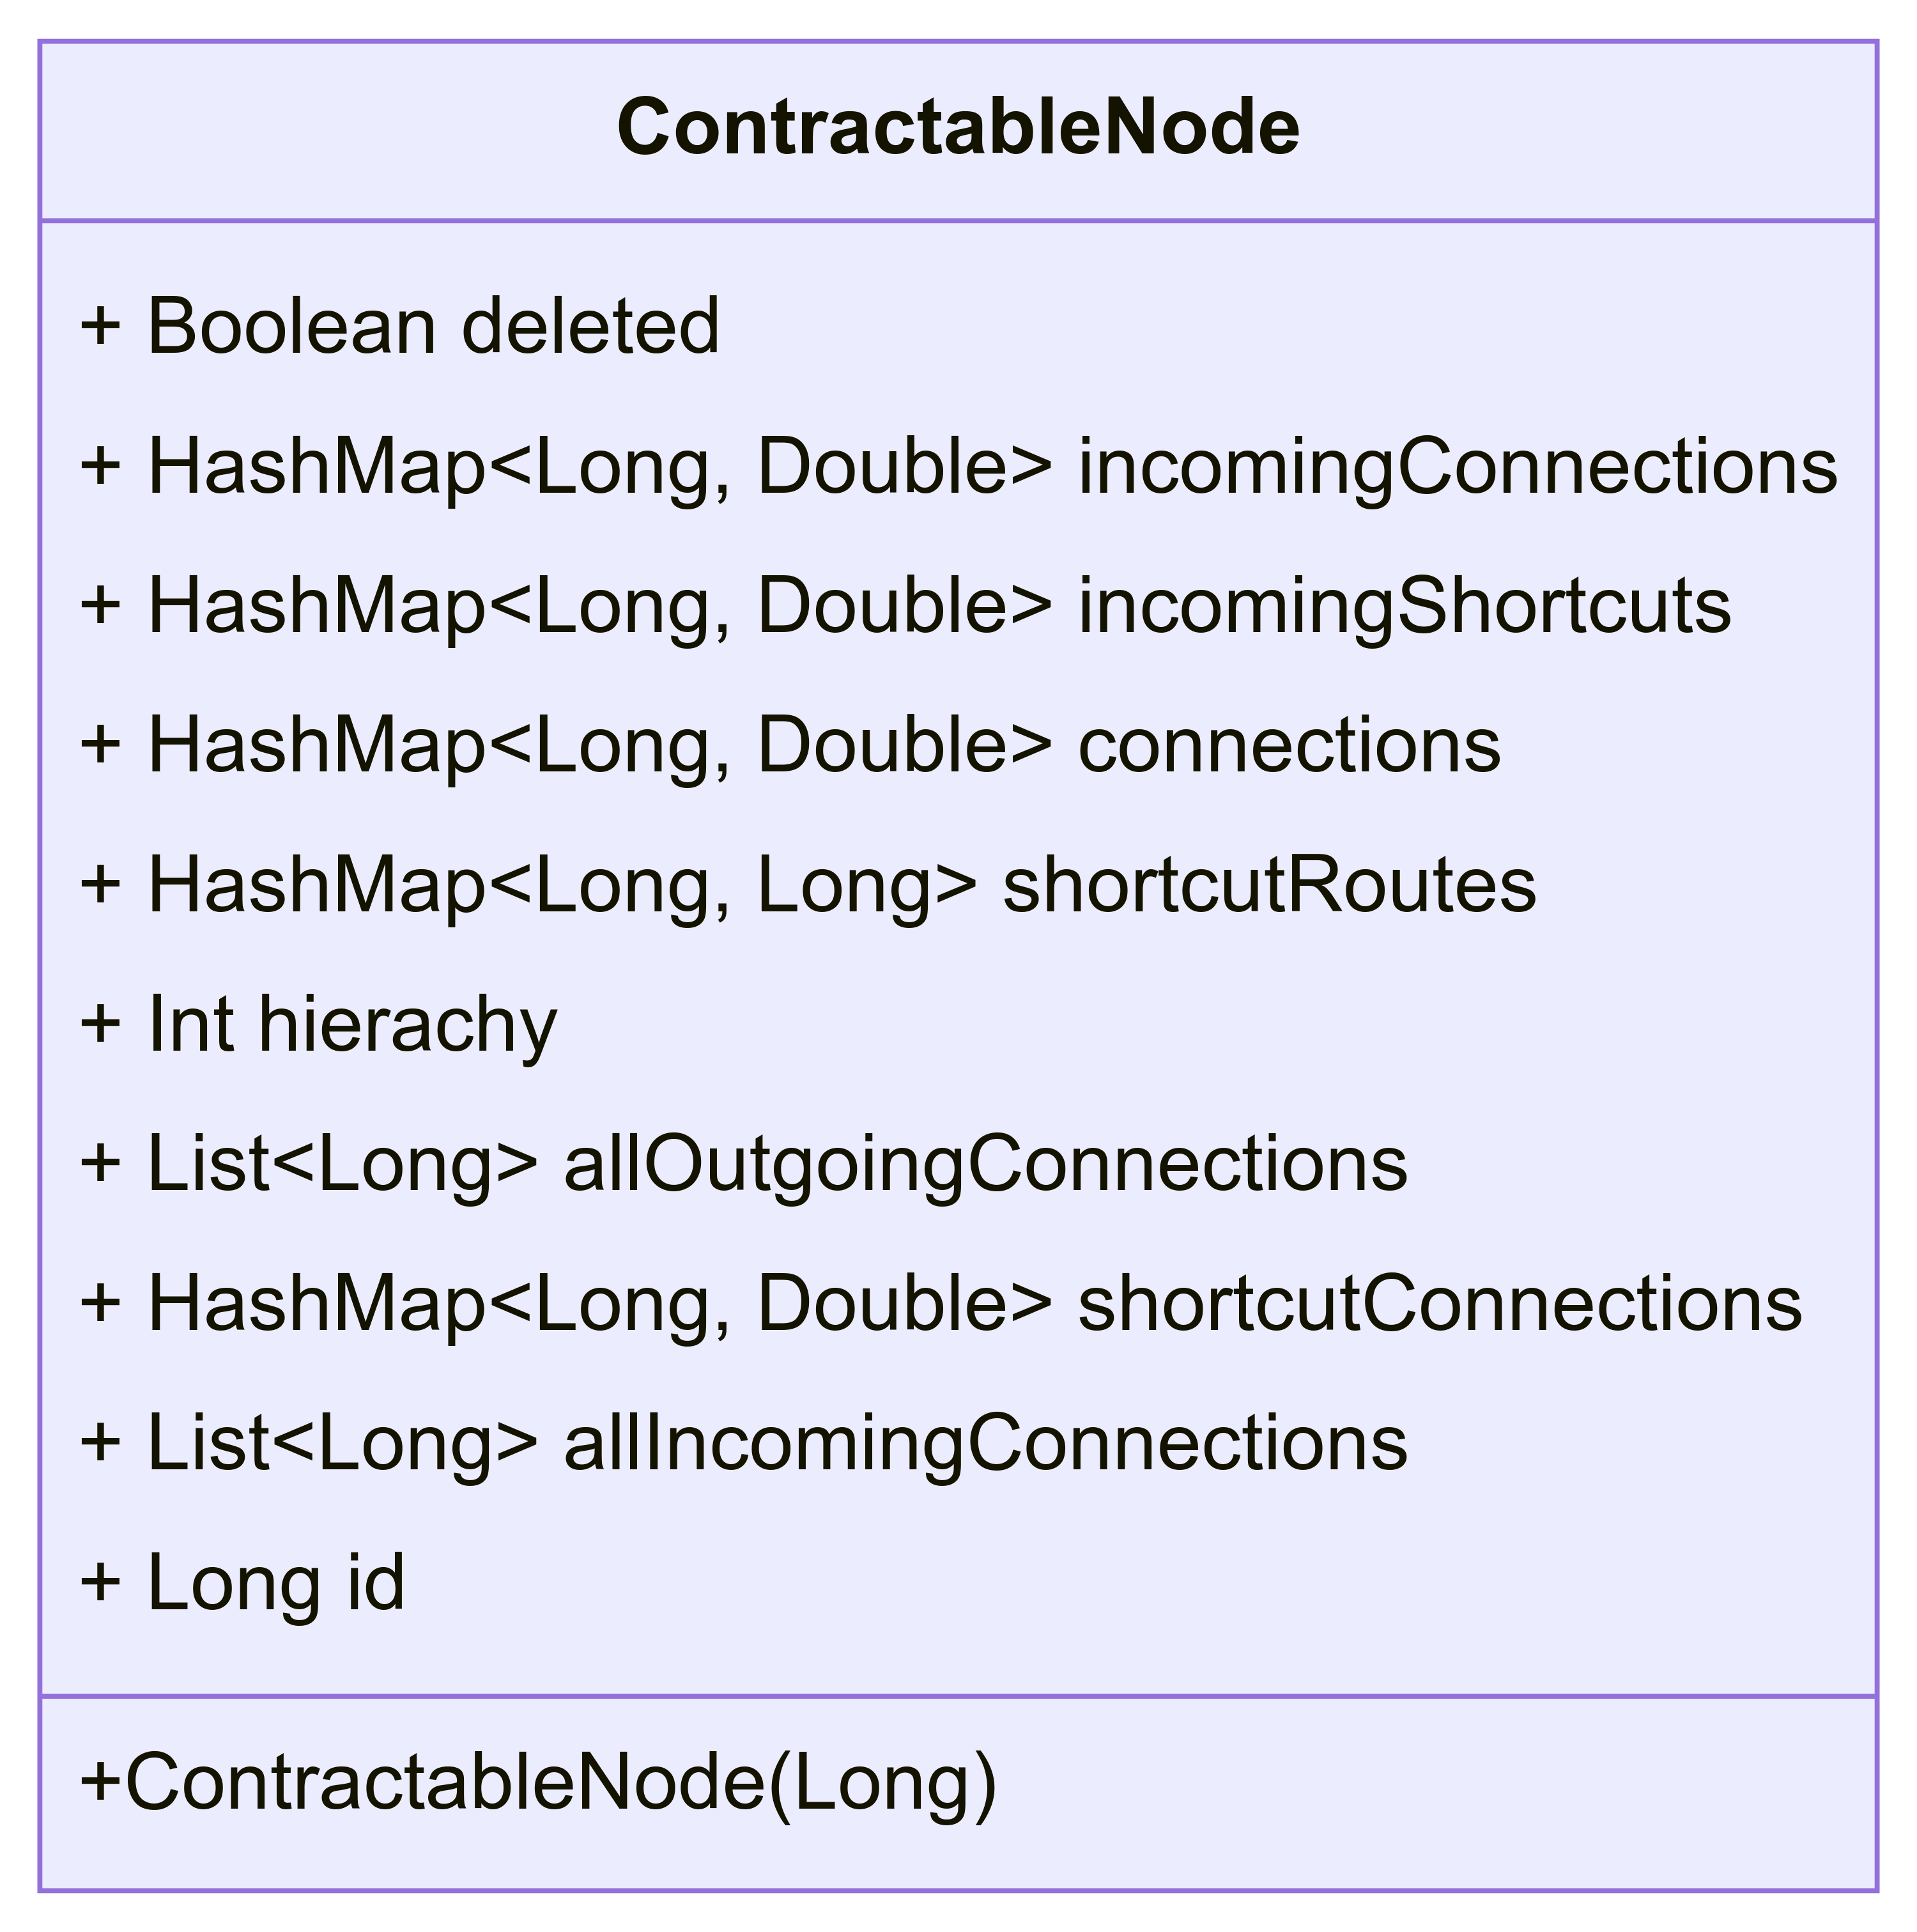
\includegraphics[width=8cm]{ContractableNode.png}
\end{center}
\caption{UML class Diagram for the \texttt{ContractableNode} subclass}
\label{ContractableNode}
\end{figure}
In order to create a contracted graph, the two functions \texttt{createGraph} and \texttt{contractGraph} must be run. \texttt{createGraph} simply copies the relevant information from the \texttt{GeographicNode} objects in the \texttt{GeographicGraph} to \texttt{ContractableNode} objects in the new object.
\texttt{contractGraph} runs the graph contraction algorithms.
\begin{lstlisting}[language=kotlin]
fun contractGraph(inputGraph: GeographicGraph) {
    println("Contracting Graph of size ${vertices.size}")
    var current = 1
    var contractionQueue = PriorityQueue<IntTuple>()
    var count = 0
    for (vertice in vertices.keys) {
        contractionQueue.add(IntTuple(vertice, getHeuristicValue(vertice, inputGraph)))
        println("There are ${contractionQueue.size} nodes left to contract")
    }
    while (contractionQueue.size != 0) {
        if (count == 40) {
            println("Recalculating Queue")
            val newQueue = PriorityQueue<IntTuple>()
            while (contractionQueue.size != 0) {
                val current = contractionQueue.poll()
                val edgeDifference = getHeuristicValue(current.id, inputGraph)
                newQueue.add(IntTuple(current.id, edgeDifference))
            }
            contractionQueue = newQueue
            count = 0
        }
        val next = contractionQueue.poll()
        val oldHeuristic = next.dist
        val newHeuristic = getHeuristicValue(next.id, inputGraph)
        if (oldHeuristic != newHeuristic) {
            count += 1
            contractionQueue.add(IntTuple(next.id, newHeuristic))
            continue
        } else {
            count = 0
        }
        contractNode(next.id, current, inputGraph)
        current += 1
        println("There are ${contractionQueue.size} nodes left to contract")
    }
    println("Contraction finished")
    for (vertice in vertices) {
        vertice.value.allOutgoingConnections =
            vertice.value.shortcutConnections.keys.union(vertice.value.connections.keys).toList()
        vertice.value.allIncomingConnections =
            vertice.value.incomingShortcuts.keys.union(vertice.value.incomingConnections.keys).toList()
    }
}
\end{lstlisting}
As mentioned in Section \ref{contractiondesign}, this function uses a priority queue and heuristics to determine which node to contract next. The items in the Queue are held in \texttt{IntTuple} objects, which are the same as \texttt{DoubleTuple} objects, but use integers instead of doubles.If the heuristic of the item has changed since being inserted into the queue,
the item is reinserted to the queue. If this happens 40 times in a row, the entire queue is recalculated. When all the nodes are contracted, they have their shortcut and normal connections unioned together. This is further preprocessing for later route finding, as before implementing this
finding unions of these sets was taking up the majority of the time used to find routes. \\
The heuristic function \texttt{getHeuristicValue} is the sum of the edge difference and the number of deleted nodes connected to a node considered for contraction. It calls \texttt{getShortest} for every incoming node to the given node. \texttt{getShortest} gives the list of outgoing nodes such that the shortest path between the incoming and outgoing node goes through the given node. 
\begin{lstlisting}[language=kotlin]
/**
* Generates a tree which can then be checked for shortest routes
* The tree is built until all neighbours of the about node are found, then queried to find if the shortest route goes through the about node
* The estimation feature enables faster estimations of edge differences by terminating the search after a given number of nodes,
* but can be disabled for the real contraction operation
*/
private fun getShortest(
    from: Long,
    about: Long,
    inputGraph: GeographicGraph,
    estimation: Boolean
): MutableList<Long> {
    val toFind = vertices[about]!!.connections.keys.union(vertices[about]!!.shortcutConnections.keys)
        .filter { x -> !vertices[x]!!.deleted }.toHashSet()
    HashSet<Long>()
    val F = PriorityQueue<DoubleTuple>()
    val dist = HashMap<Long, Double>()
    val prev = HashMap<Long, Long>()
    var numsettled = 0
    dist[from] = 0.0
    prev[from] = -1
    var u: Long
    var toAdd = DoubleTuple(from, 0.0)
    F.add(toAdd)
    while (F.size != 0) {
        val item = F.poll()
        u = item.id
        if (dist[u] != item.dist) continue
        toFind.remove(u)
        numsettled += 1
        for (neighbour in vertices[u]!!.connections.keys) {
            var alt = dist[u]!! + vertices[u]!!.connections[neighbour]!!
            if (!dist.containsKey(neighbour) || alt < dist[neighbour]!!) {
                toFind.remove(neighbour)
                dist[neighbour] = alt
                prev[neighbour] = u
                toAdd = DoubleTuple(neighbour, dist[neighbour]!!)
                F.add(toAdd)
            }
        }
        if (toFind.size == 0 || (numsettled == 10000 && estimation)) break
    }
    val shortestThrough = mutableListOf<Long>()
    for (i in vertices[about]!!.connections.keys.union(vertices[about]!!.shortcutConnections.keys)
        .filter { x -> !vertices[x]!!.deleted }) {
        if (i == from) continue
        if (!prev.containsKey(i)) shortestThrough.add(i) //i has not been reached because contraction has been terminated early, therefore a shortcut is necessary
        else {
            val route = inputGraph.solution(i, prev)
            if (route.contains(about)) shortestThrough.add(i) //The shortest route goes through the node therefore a shortcut is necessary
        }
    }
    return shortestThrough
}
\end{lstlisting}
In order to speed up the contraction process, a settled node limit of 10000 is imposed for estimating the edge difference, but not for the actual contraction of nodes, as this limit would result in unecessary shortcuts.
\newpage
\subsubsection{Graph Querying}
Once the graph has been sucessfully contracted, all that remains is to allow for route finding. 
The \texttt{findRoute} function implements a complete bidirectional dijkstra search in the reduced search space to find a node that is known to be on the minimum path.
\begin{lstlisting}[language=kotlin]
/**
    * Finds the route using contraction hierachies.
    * First the set of nodes with a higher hierarchy from the from node are calculated
    * Then the set of nodes with a higher hierachy from the to node (backwards) are calculated
    * Then the intersection of the set of settled nodes is found and the minimum found
    * Then the route is created by iteratively looking up the shortcuts
    */
fun findRoute(from: Long, to: Long, inputGraph: GeographicGraph, showVisited: Boolean): List<Long> {
    //first we generate the upwards and downwards search spaces using simple queues
    val Q: Queue<Long> = LinkedList<Long>()
    val upwardsSpace = HashSet<Long>()
    val downSpace = HashSet<Long>()
    Q.add(from)
    while (Q.size != 0) {
        val current = Q.poll()
        upwardsSpace.add(current)
        for (neighbour in vertices[current]!!.allOutgoingConnections) {
            if (vertices[neighbour]!!.hierachy > vertices[current]!!.hierachy && !upwardsSpace.contains(neighbour)) {
                Q.add(neighbour)
            }
        }
    }
    Q.add(to)
    while (Q.size != 0) {
        val current = Q.poll()
        downSpace.add(current)
        for (neighbour in vertices[current]!!.allOutgoingConnections) {
            if (vertices[neighbour]!!.hierachy > vertices[current]!!.hierachy && !downSpace.contains(neighbour)) {
                Q.add(neighbour)
            }
        }
    }
    var F = PriorityQueue<DoubleTuple>()
    val settledFrom = HashSet<Long>()
    val dist = HashMap<Long, Double>()
    val prev = HashMap<Long, Long>()
    var u: Long
    var toAdd = DoubleTuple(from, 0.0)
    dist[from] = 0.0
    F.add(toAdd)
    while (F.size != 0) {
        val item = F.poll()
        u = item.id
        if (dist[u] != item.dist) continue
        settledFrom.add(u)
        for (neighbour in vertices[u]!!.allOutgoingConnections) {
            if (!upwardsSpace.contains(neighbour)) continue
            var cost: Double =
                if (vertices[u]!!.connections.containsKey(neighbour)) vertices[u]!!.connections[neighbour]!!
                else vertices[u]!!.shortcutConnections[neighbour]!!
            val alt = cost + dist[u]!!
            if (!dist.containsKey(neighbour) || alt < dist[neighbour]!!) {
                dist[neighbour] = alt
                prev[neighbour] = u
                toAdd = DoubleTuple(neighbour, dist[neighbour]!!)
                F.add(toAdd)
            }
        }
    }
    F = PriorityQueue<DoubleTuple>()
    val settledTo = HashSet<Long>()
    val distTo = HashMap<Long, Double>()
    val prevTo = HashMap<Long, Long>()
    distTo[to] = 0.0
    toAdd = DoubleTuple(to, 0.0)
    F.add(toAdd)
    while (F.size != 0) {
        val item = F.poll()
        u = item.id
        if (distTo[u] != item.dist) continue
        settledTo.add(u)
        for (neighbour in vertices[u]!!.allIncomingConnections) {
            if (!downSpace.contains(neighbour)) continue
            var cost: Double =
                if (vertices[u]!!.incomingConnections.containsKey(neighbour)) vertices[u]!!.incomingConnections[neighbour]!!
                else vertices[u]!!.incomingShortcuts[neighbour]!!
            val alt = cost + distTo[u]!!
            if (!distTo.containsKey(neighbour) || alt < distTo[neighbour]!!) {
                distTo[neighbour] = alt
                prevTo[neighbour] = u
                toAdd = DoubleTuple(neighbour, distTo[neighbour]!!)
                F.add(toAdd)
            }
        }
    }
    var minimumNode: Long = -1
    var minimumCost = Double.MAX_VALUE
    for (i in settledTo.intersect(settledFrom)) {
        if (dist[i]!! + distTo[i]!! - inputGraph.vertices[i]!!.weight < minimumCost) {
            minimumNode = i
            minimumCost = dist[i]!! + distTo[i]!! - inputGraph.vertices[i]!!.weight
        }
    }
    println(minimumCost)
    return if (showVisited) settledTo.intersect(settledFrom).toList()
    else deContractRoute(minimumNode, prev, prevTo)
}
\end{lstlisting}
The implementation of this function is fairly standard, it just consists of two dijkstra searches in reduced search spaces and a call to \texttt{deContractRoute}. \texttt{deContractRoute} works both backwards and forwards from the minimum node to gather the whole route, then it fills in all of the shortcuts.
\begin{lstlisting}[language=kotlin]
private fun deContractRoute(minimumNode: Long, prev: HashMap<Long, Long>, prevTo: HashMap<Long, Long>): List<Long> {
    val route = mutableListOf<Long>(minimumNode)
    while (prev.containsKey(route[0]) && prev[route[0]]!! != -1L) {
        route.add(0, prev[route[0]]!!)
    }
    while (prevTo.containsKey(route.last()) && prevTo[route.last()]!! != -1L) {
        route.add(prevTo[route.last()]!!)
    }
    return unpackRoute(route)
}

private fun unpackRoute(route: MutableList<Long>): MutableList<Long> {
    while (true) {
        var finished = true
        for (i in 1 until route.size) {
            if (route[i - 1] == -1L) continue
            val current = vertices[route[i - 1]]!!
            if (current.shortcutConnections.containsKey(route[i])) {
                route.add(i, current.shortcutRoutes[route[i]]!!)
                finished = false
                break
            }
        }
        if (finished) break
    }
    return route
}
\end{lstlisting}
\texttt{unpackRoute} operates in a similar manner to a bubble sort, repeatedly iterating through the list until it is known that it contains no shortcuts. 
\section{User Interface}
The user interface is written in the \texttt{Main.kt} file. It is defensively programmed, to protect from user error, and the code is shown in the Appendix. It allows for an input loop. An example usage is shown in Figure \ref{interface}.
\begin{figure}[t]
\begin{center}
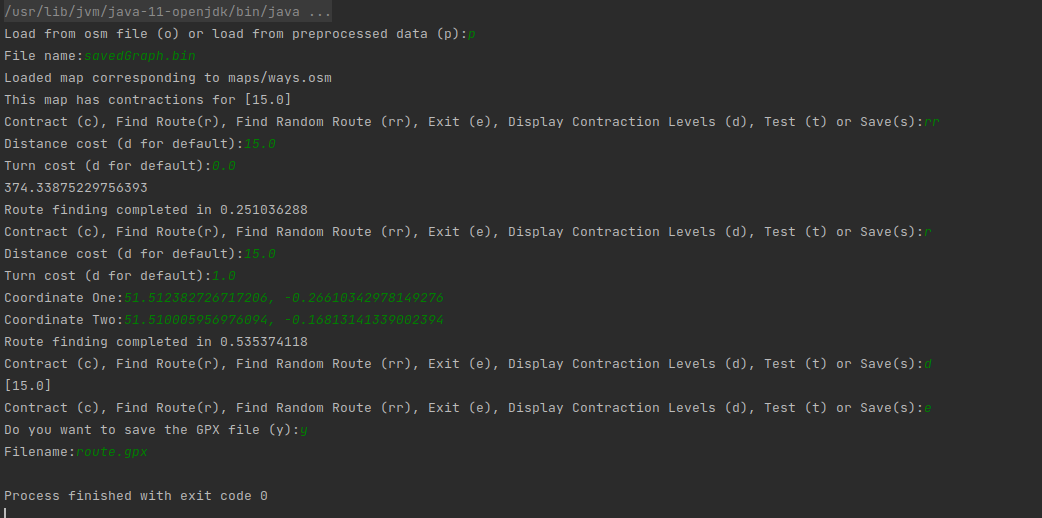
\includegraphics[width=8cm]{interface.png}
\end{center}
\caption{The interface for my program}
\label{interface}
\end{figure}
\newpage
\section{Serialisation}
In order to serialise objects of a certain class in kotlin, the class and all of the properties of the class must be serialisable. Kotlin data structures, like HashMaps and HashSets are all serialisable.
The only data structure that was not serialisable was the R*Tree, so this had to be marked as Transient so that the serialiser would not complain, and then regenerated by calling \texttt{setupRTree} upon deserialisation.
\begin{lstlisting}[language=kotlin]
@Serializable
class GeographicGraph {
    var vertices: HashMap<Long, GeographicNode> = HashMap()
    var safeNodes = HashSet<Long>() //nodes that are known to be safe
    var slowNodes = HashSet<Long>()
    var contractedGraphs = HashMap<Double, ContractableGraph>()

    @Transient
    lateinit var nodeTree: RTree<Long, Geometry>
\end{lstlisting}
When a method is deserialised, the intialisation method is run, so I had to move the functionality of these into other functions to stop things incorrectly being added twice upon deserialisation.
The \texttt{OpenStreetMap} class has a init method, but this checks to see if the \texttt{cyclableGraph} has already been created, and if so does nothing.
\begin{lstlisting}[language=kotlin]
init {
    if (cyclableGraph.vertices.size == 0) {
        println("Parsing XML")
        parseXML(filename)
        println("Pruning Disconnected")
        cyclableGraph.pruneDisconnected()
        println("Creating rTree")
        cyclableGraph.setupRTree()
        println("Gathering weights")
        cyclableGraph.gatherWeights()
        for (node in cyclableGraph.safeNodes)
            cyclableGraph.vertices[node]?.weight = 0.0
    }
}
\end{lstlisting}
\newpage
\chapter{Testing}
I employed 3 major strategies to test my Project.
\begin{enumerate}
    \item Comprehensive unit testing. Tests are defined for every major function in code, and run regularly. This helps ascertain that the code works, and also helps to ensure that bugs are not introduced during development.
    \item Human Testing. Essentially a human uses the program and ascertains that the program complies with specification points and does not crash when the user does unexpected things.
    \item Performance Testing. In order to ascertain that the program runs at an acceptable speed, automated performance tests measure the speed of certain functions.
\end{enumerate}
\section{Creating a test area}
Some operations, especially preprocesing, take a long time to execute. As the unit tests will be run many times, it makes sense to define a smaller test area for some operations. I created a GeoJSON file, and used it to cut out a smaller area of london, called \texttt{testarea.osm}.
\section{Unit Testing}
The basic idea of unit testing is to test that all functions do what they should do. Where possible, I manually worked out what they should do and set this as the condition for the test.
\begin{figure}[t]
    \begin{center}
        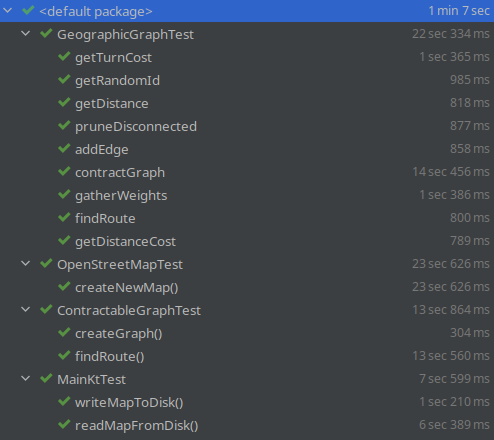
\includegraphics[height=4cm]{test.png}
        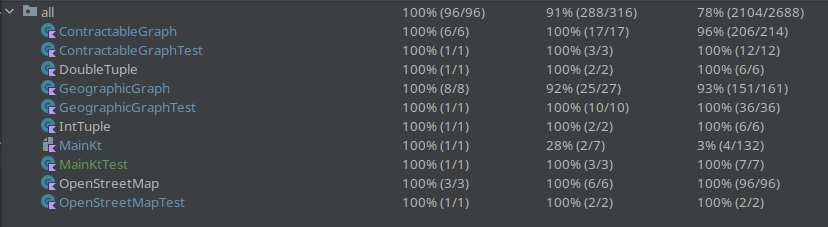
\includegraphics[height=4cm]{coverage.png}
    \end{center}
    \caption{Unit tests running successfully, as well as code coverage stats}
    \label{testsuccess}
\end{figure}
\small{
\begin{longtable}[c]{|c|p{6cm}|c|c|}
    \hline
    \multicolumn{4}{| c |}{Unit Testing Table}\\
    \hline
    Test Coverage & Description & Type & Works?\\
    \hline
    \endfirsthead
   
    \hline
    \multicolumn{4}{|c|}{Continuation of Unit Testing Table}\\
    \hline
    Test Coverage & Description & Type & Works?\\
    \hline
    \endhead
   
    \hline
    \endfoot

    \texttt{GeographicGraph.getDistance} & At the equator, a degree of longitude is approximately 111km. This function calculates a degree of longitude at the equator and checks that it is close to 111km & Equals & \checkmark\\
    \hline
    \texttt{GeographicGraph.getRandomId} & A random id is sucessfully generated which is in the graph set of vertices & Boolean & \checkmark\\
    \hline
    \texttt{GeographicGraph.addEdge} & Add both directed and undirected edges to a graph, and makes sure they are added correctly & Boolean & \checkmark\\
    \hline
    \texttt{GeographicGraph.gatherWeights} & Set all weights in the graph to 0, gather them again, and check for right value & Equals & \checkmark\\
    \hline 
    \texttt{GeographicGraph.getDistanceCost} & Checks that the calculated distance cost between two close nodes is as expected & Equals & \checkmark\\
    \hline
    \texttt{GeographicGraph.pruneDisconnected} & Runs the function on the graph, and checks that nothing changes as it has been run before & Equals & \checkmark\\
    \hline
    \texttt{GeographicGraph.getTurnCost} & Runs the turn cost function on nodes in a straight road, and around a 90 degree turn & Equals & \checkmark\\
    \hline
    \texttt{GeographicGraph.contractGraph} & Runs the contraction function on the graph & No Errors & \checkmark\\
    \hline
    \texttt{GeographicGraph.findRoute} & Runs the route finding algorithm and checks the total distance & Equals & \checkmark\\
    \hline
    \texttt{ContractableGraph.createGraph} & Creates a new contractable graph & No Errors & \checkmark\\
    \hline
    \texttt{ContractableGraph.findRoute} & Creates and contracts a \texttt{ContractableGraph} instance, then checks the route found has the right cost. & Equals & \checkmark\\
    \hline
    \texttt{OpenStreetMap} & Creates a new \texttt{OpenStreetMap} instance & No Errors & \checkmark\\
    \hline
    \texttt{MainKt.writeMapToDisk} & Writes an OSM file to disk, reads it back, and checks that the size of the graphs is the same & Equals & \checkmark\\
    \hline
    \texttt{MainKt.writeObjectToDisk} & Writes an OSM file to disk, reads it back, and checks that the size of the graphs is the same & Equals & \checkmark\\
\end{longtable}
}
As shown in Figure \ref{testsuccess}, all of these tests ran successfully, and had relatively high code coverage considering that most of the lines in \texttt{Main.kt}
cannot be easily unit tested as they rely on user input. 
\section{Human Testing}
I also used human testing to make sure that the program runs as specified. These tests mostly check that code does not break when given difficult inputs, but also that it conforms to other specification points.
I used two types of tests: Normal tests, where everything should work, and breaking tests, where the program should not crash and give an expected output. 
\small{
\begin{longtable}[c]{|c|p{6cm}|c|c|c|}
    \hline
    \multicolumn{5}{| c |}{Human Testing Table}\\
    \hline
    Covered Specification Point & Description & Type & Evidence & Works?\\
    \hline
    \endfirsthead
    \hline
    \endfoot
   
    \hline
    \multicolumn{5}{|c|}{Continuation of Human Testing Table}\\
    \hline
    Covered Specification Point & Description & Type & Evidence & Works?\\
    \hline
    \endhead
    \ref{downloadaccidents}  & Run the \texttt{download.py} script and check that accidents are properly stored. & Normal & & \checkmark\\
    \hline
    \ref{parseaccidents} \& \ref{storeaccidents} & Run \texttt{parse.py} and verify that the \texttt{output.json} file is created correctly using \texttt{display.py} & Normal & & \checkmark\\
    \hline
    \ref{item-one} \& \ref{item-two} \& \ref{item-three} \& \ref{item-four} & Run the program, and select a \texttt{.osm} file to parse, and verify it is parsed correctly by finding a route between two points. & Normal & & \checkmark\\
    \hline
    \ref{item-five} \& \ref{item-six} \& \ref{item-seven} \& \ref{item-eight} \& \ref{item-fifteen}& Find a route between two points, and evaluate whether following it would be safe, legal, \&possible, by following the route. & Normal & Appendix \ref{Real World Testing} & \checkmark\\
    \hline
    \ref{item-ten} & Load a \texttt{.osm} file, contract the graph, then execute and check a \texttt{findRoute} query on that graph. & Normal & & \checkmark\\
    \hline
    \ref{item-eleven} & Run a contracted and non contracted query on the same graph, and verify that they overlap. & Normal & & \checkmark\\
    \hline
    \ref{item-thirteen} \& \ref{item-fourteen} & Attempt to cause a crash by inputting illegal inputs. Verify that this fails & Illegal & & \checkmark\\
    \hline
    \ref{item-sixteen} & Create and then save a map. Load the map back into memory and verify that route finding on it still works & Normal & & \checkmark
\end{longtable}
}
\section{Performance Testing}
\chapter{Evaluation}
\newpage
\appendix
\appendixpage
\addappheadtotoc
\chapter{Evidence for Human Testing}
\chapter{Real World Testing}
\label{Real World Testing}
In order to  
\chapter{Program Source Code}
\newpage
\addcontentsline{toc}{chapter}{References}
\printbibliography
\label{end}
\end{document}     